%%%%% DOCUMENT CLASS
\documentclass[11pt]{article}

%%%%% IMPORTING PACKAGES
\usepackage{geometry} % page format
\usepackage{setspace} % page format
\usepackage{amsmath, amsthm, amssymb} % math stuff
\usepackage{mathtools} % math stuff
\usepackage{mathrsfs} % math stuff
\usepackage{empheq} % math stuff
\usepackage{cancel} % math stuff
\usepackage{tikz} % for making figures
\usepackage{graphicx} % for figures
\usepackage{placeins} % for figure placement
\usepackage{caption, subcaption} % for figures
\usepackage{enumitem} % for lists
\usepackage{verbatim} % for pasting .txt files
\usepackage{array} % table stuff
\usepackage{threeparttable} % table stuff
\usepackage{tabularx} % table stuff
\usepackage{multirow} % table stuff
\usepackage{colortbl} % table stuff
\usepackage{booktabs} % table stuff
\usepackage{pdfpages} % for importing pdfs
\usepackage{hyperref} % for hyperlinks
\usepackage{titletoc} % for TOC
\usepackage[table,dvipsnames]{xcolor} % for text coloring
\usepackage[backend=biber,sorting=none,style=numeric-comp]{biblatex} % for references
\usepackage{lipsum} % for filler
\usepackage{comment} % for comments
\usepackage{minted} % for code listings
% \usepackage{listings} % for code listings (alternative option)

%%%%% CONFIGURING PACKAGE SETTINGS
% paper size
\geometry{letterpaper,left=1in,top=1in,right=1in,bottom=1in}

% line spacing
% \singlespacing
\onehalfspacing
% \doublespacing
% \setstretch{1.25}

% graphics stuff
\graphicspath{ {./Figures/} }
\allowdisplaybreaks[1]

% links
\hypersetup{colorlinks=true, linkcolor=red, filecolor=magenta, urlcolor=black, citecolor=blue}

% adding bib
\addbibresource{bib.bib}

% list customization
\setlist[enumerate]{itemsep=1pt}

%%%%% CREATING CUSTOM COMMANDS
% custom page numbering
\newcommand{\mainmatter}{\clearpage\setcounter{page}{1}\pagenumbering{arabic}}
\newcommand{\appendixpagenumbering}{\clearpage\pagenumbering{arabic}\renewcommand{\thepage}{A-\arabic{page}}}

% TOC customization
\newcommand\innercontentsname[1]{%
Contents for section~\ref{#1}}

% custom table columns
\newcolumntype{P}[1]{>{\centering\arraybackslash}p{#1}}
\newcolumntype{M}[1]{>{\centering\arraybackslash}m{#1}}
\newcolumntype{R}[1]{>{\raggedleft\arraybackslash}m{#1}}
\renewcommand\tabularxcolumn[1]{m{#1}}

% whatever math operators we need
\DeclareMathOperator{\sgn}{sgn}
\DeclareMathOperator{\acos}{acos}
\DeclareMathOperator{\atantwo}{atan2}
\DeclareMathOperator{\spec}{Spec}
\DeclareMathOperator{\rank}{Rank}

% math configuration
\setcounter{MaxMatrixCols}{12}

%%%%% DOCUMENT
\begin{document}

%%%%% TITLE PAGE
\begin{titlepage}
\begin{center}
    \vspace*{\fill}
    {\Huge Quadrotor RGBD-Camera Optimal Target Tracking}\\
    {\large Final Project Report}

    \vspace{4\baselineskip}
    Daniel Whitman\\
    Robot Perception (MAE 5810)\\
    12/07/2026
\end{center}

\vspace{4\baselineskip}
\noindent \textbf{ABSTRACT:}
\noindent Quadrotors are becoming increasingly prevalent in robotic perception applications due to their maneuverability, stability, and generalized capabilities. This project mathematically models a quadrotor with a front-mounted RGBD-camera sensor for use in optimal target tracking and following around an environmental obstacle. Object detection and bounding box generation were used to estimate the target's pixels in the camera image to then reconstruct the estimated target position and velocity dynamics, thus providing a reference trajectory for a discrete TV-LQR optimal controller. The model was found to be able to effectively track and follow the target as it moved through the world, even after the target was entirely occluded by an environmental obstacle.

\vspace*{\fill}
\end{titlepage}

%%%%% ABSTRACT PAGE
% \clearpage
% \pagenumbering{gobble}
% \section*{ABSTRACT}
% \noindent Words

%%%%% ACTUAL REPORT
\mainmatter
\section{INTRODUCTION}\label{sec:intro}
In recent years, quadrotors have provided an excellent platform for robotic perception, seeing deployment and use in many applications, such as mapping, search-and-rescue, exploration, surveillance, inspection, surveying, 3D reconstruction, and others \cite{Michael2012Cmoae,Ribeiro2020UAVL,Sun2024SFaLU,Zhang2022ANIAE,Zhong2022IDFMA}. Their high maneuverability, small aerial footprint, natural stability, and generalizable payload capabilities allow for a diverse use of quadrotors with a variety of sensors specific to the desired task. Because of their aerial nature, they can navigate through environments that would otherwise be difficult for land-based robots and provide ``eye in the sky'' support for both people and other robotic systems alike, earning their place as a valuable asset in the perception community.

In this project, a quadrotor with a front-mounted RGBD-camera module will be simulated in an active perception environment to optimally track and follow a target as it moves around an obstacle. The goal is to use an optimal controller to ensure that the quadrotor is able to maintain tracking of the target even with environmental occlusions. Section \ref{sec:theory} (Theory and Methods) presents the mathematical model for the quadrotor-camera optimal control system that describes how the system is able to effectively track the target using only RGBD-camera sensor measurements. Section \ref{sec:procedure} (Procedure) describes the simulation framework and modeling, and explains how the tracking was achieved. Section \ref{sec:results} (Results) demonstrates the outcome of the tracking control algorithm through simulation, illustrating how the quadrotor is able to effectively measure the target's dynamic state through tracking. Finally, Section \ref{sec:conclusion} (Conclusions) summarizes the work and presents future directions for improvement.

\section{THEORY AND METHODS}\label{sec:theory}

\subsection{MATHEMATICAL PRELIMINARIES}
Vectors are given with \textbf{bold} lower-case letters $(\mathbf x)$, matrices are given with capital letters $(K)$, components are either given with sub-scripted lower-case letters $(x_1)$ or plain lower-case letters $(x)$, and frames are either given as sub/superscripts $({}^A,\ {}_B)$ or in braces $(\{A\})$. A given vector $\mathbf x_A^B$ with \textit{both} a capital subscript and a superscript denotes the vector of frame ${}^B$ with respect to frame ${}_A$. Therefore, $\mathbf x_W^Q$ is the state vector of the quadrotor frame ${}^Q$ with respect to the world frame ${}_W$. Similarly, a homogeneous transformation matrix $T_A^B$ represents the transformation of frame ${}^B$ with respect to frame ${}_B$, so $T_W^Q$ represents the transformation of the quadrotor frame ${}^Q$ with respect to the world frame ${}_W$, such that, for example, $\mathbf x_W^C=T_W^Q\mathbf x_Q^C$. With this notation, the inverse transformation $(T_W^Q)^{-1}\equiv T_Q^W$. A vector $\mathbf x_A$ with \textit{only} a subscript or a vector $\mathbf x_A^b$ with mixed-case sub/super scripts denotes a vector specific to object ${}_A$ with note ${}^b$. For example, $\mathbf x_T^e$ is the estimated (${}^e$) target (${}_T$) position vector in the world frame.

\subsection{SENSOR MATHEMATICAL MODEL}
For this model, the camera sensor is located at the front of a quadrotor. Therefore, the ``panning'', ``tilting'', and ``rotating'' of the sensor are due to the motion of the quadrotor itself, and so to fully capture the mathematical model of the sensor, the dynamics of the quadrotor must be known. The equations of motion for the quadrotor are taken from \cite{Ferrari20221IDPaC} are are represented as the system:
\begin{align}
    \dot u&=(vr-wq)+g\sin\theta & \dot x&=(\sin\psi\sin\phi+\cos\phi\sin\theta\cos\phi)\frac{u_1}{m}\nonumber\\
    \dot v&=(wp-ur)-g\sin\phi\cos\theta & \dot y&=(-\cos\psi\sin\phi+\sin\psi\sin\theta\cos\phi)\frac{u_1}{m}\nonumber\\
    \dot w&=(uq-vp)-g\cos\phi\cos\theta+\frac{u_1}{m} & \dot z&=-g+(\cos\theta\cos\phi)\frac{u_1}{m}\nonumber\\
    \dot p&=\frac{I_{yy}-I_{zz}}{I_{xx}}qr-\frac{J_R}{I_{xx}}q\Omega+\frac{u_2}{I_{xx}} & \dot\phi&=p+(q\sin\phi+r\cos\phi)\tan\theta\nonumber\\
    \dot q&=\frac{I_{zz}-I_{xx}}{I_{yy}}pr-\frac{J_R}{I_{yy}}p\Omega+\frac{u_3}{I_{yy}} & \dot\theta&=q\cos\phi-r\sin\phi\nonumber\\
    \dot r&=\frac{I_{xx}-I_{yy}}{I_{zz}}pq+\frac{u_4}{I_{zz}} & \dot\psi&=(q\sin\phi+r\cos\phi)/\cos\theta\,,\label{eqn:dynamics}
\end{align}
where
\begin{align}
    u_1&=C_T(\Omega_1^2+\Omega_2^2+\Omega_3^2+\Omega_4^2) & u_2&=C_T\ell(\Omega_4^2-\Omega_2^2)\nonumber\\
    u_3&=C_T\ell(\Omega_3^2-\Omega_1^2) & u_4&=C_D(\Omega_2^2+\Omega_4^2-\Omega_1^2-\Omega_3^2)\nonumber\\
    \Omega&=-\Omega_1+\Omega_2-\Omega_3+\Omega_4\,.\label{eqn:uforces}
\end{align}

From these dynamics, the important quantities to consider for the sensor are the Euler angles ($\phi,\theta,\psi$) defining the rotation matrix
\begin{align}\label{eqn:R}
    R=R_{z\psi}R_{y\theta}R_{x\phi}&=\begin{pmatrix}
        c_\theta c_\psi & -c_\phi s_\psi+s_\phi s_\theta c_\psi & s_\phi s_\psi+c_\phi s_\theta c_\psi\\
        c_\theta s_\phi & c_\phi c_\psi+s_\phi s_\theta s_\psi & -s_\phi c_\psi+c_\phi s_\theta s_\psi\\
        -s_\theta & s_\phi c_\theta & c_\phi c_\theta
    \end{pmatrix}\,,
\end{align}
the position of the quadrotor with respect to the world frame $\mathbf x_W^Q=(x,y,z)^T$, the velocity of the quadrotor with respect to the world frame $\dot{\mathbf x}_W^Q=(\dot x,\dot y,\dot z)^T$, and the angular rotation about the quadrotor body frame $\boldsymbol\omega_Q^Q=(p,q,r)^T$. With these, we can define the transformation of the quadrotor frame $\{Q\}$ with respect to the world frame $\{W\} $ with (\ref{eqn:R}) as
\begin{align}\label{eqn:TWQ}
    T_W^Q&=\begin{pmatrix}
        R & \mathbf x_W^Q\\\mathbf0 & 1
    \end{pmatrix}\,.
\end{align}

Now, we can consider attaching a camera frame somewhere to the body of the quadrotor. We can define the transformation of the camera frame $\{C\}$ with respect to the quadrotor frame $\{Q\}$ as
\begin{align}\label{eqn:TQC}
    T_Q^C&=\begin{pmatrix}
        R_Q^C & \mathbf b_Q^C\\\mathbf0 & 1
    \end{pmatrix}\,,
\end{align}
where $\mathbf b_Q^C$ is the translation of the camera frame with respect to the quadrotor frame and $R_Q^C$ is the rotation of the camera frame with respect to the quadrotor frame, such that, by convention, the camera frame $z$-axis points along the direction of perception, the camera frame $x$-axis points horizontally in the image, and the camera frame $y$-axis points vertically down in the image. Note, both of these quantities are \textit{constant} as the camera is fixed to the quadrotor body.

Next, given the position of a target in the world frame $\mathbf x_T=(x_T,y_T,z_T,1)^T$ (homogeneous coordinates), we can find is position in the camera frame using (\ref{eqn:TWQ}) and (\ref{eqn:TQC}) as
\begin{align}
    \mathbf q_T&=(T_W^QT_Q^C)^{-1}\mathbf x_T=(T_Q^C)^{-1}(T_W^Q)^{-1}\mathbf x_T=T_C^QT_Q^W\mathbf x_T\nonumber\\
    \mathbf q_T&=\begin{pmatrix}
        (R_Q^C)^T & -(R_Q^C)^T\mathbf b_Q^C\\\mathbf0 & 1
    \end{pmatrix}\begin{pmatrix}
        R^T & -R^T\mathbf x_W^Q\\\mathbf0 & 1
    \end{pmatrix}\mathbf x_T\nonumber\\
    \mathbf q_T&=\begin{pmatrix}
        (R_Q^C)^TR^T & -(R_Q^C)^TR^T\mathbf x_W^Q-(R_Q^C)^T\mathbf b_Q^C\\\mathbf0 & 1
    \end{pmatrix}\mathbf x_T\nonumber\\
    \mathbf q_T&\equiv T_C^W\mathbf x_T\,.\label{eqn:qT}
\end{align}

With that, we can then use the pinhole camera model to find the target position on the projection plane using pixel homogeneous coordinates as
\begin{align}
    \mathbf p_T=\begin{pmatrix}
        wu\\wv\\w\\1
    \end{pmatrix}&=\begin{pmatrix}
        f_x & 0 & u_0 & 0\\
        0 & f_y & v_0 & 0\\
        0 & 0 & 1 & 0\\
        0 & 0 & 0 & 1
    \end{pmatrix}\mathbf q_T\nonumber\\
    \mathbf p_T&\equiv K\mathbf q_T\,,\label{eqn:pT}
\end{align}
where $u$ and $v$ are the pixel coordinates in the image plane, $w$ is the normalization depth, $f_x$ and $f_y$ are the focal lengths in the camera's $x$ and $y$ directions, and $u_0$ and $v_0$ are the camera's central principal points in the camera's $x$ and $y$ directions.

From (\ref{eqn:pT}), we can calculate the pixel coordinates of the target as
\begin{align}
    wu&=f_xq_x+u_0q_z & wv&=f_yq_y+v_0q_z & w=q_z\nonumber\\
    u&=\frac{f_xq_x}{q_z}+u_0 & v&=\frac{f_yq_y}{q_z}+v_0\label{eqn:pixels}
\end{align}

We can then combine (\ref{eqn:qT}) and (\ref{eqn:pT}) to find the target position in the camera sensor's plane from its position in the world frame as
\begin{align}
    \mathbf p_T&=\begin{pmatrix}
        f_x & 0 & u_0 & 0\\
        0 & f_y & v_0 & 0\\
        0 & 0 & 1 & 0\\
        0 & 0 & 0 & 1
    \end{pmatrix}\begin{pmatrix}
        (R_Q^C)^TR^T & -(R_Q^C)^TR^T\mathbf x_W^Q-(R_Q^C)^T\mathbf b_Q^C\\\mathbf0 & 1
    \end{pmatrix}\mathbf x_T\nonumber\\
    \mathbf p_T&\equiv KT_C^W\mathbf x_T\,.\label{eqn:PTcomp}
\end{align}

Now, for a moving target with $\mathbf v_T=\dot{\mathbf x}_T$ and/or a moving quadrotor with velocity $\dot{\mathbf x}_W^Q$, it will cause the target to move in the projection plane according to
\begin{align}\label{eqn:PTd}
    \dot{\mathbf p}_T&=K(\dot T_C^W\mathbf x_T+T_C^W\mathbf v_T)\,,
\end{align}
with $\dot T_C^W$ derived as
\begin{align}
    \dot T_C^W&=\frac{d}{dt}\begin{pmatrix}
        (R_Q^C)^TR^T & -(R_Q^C)^TR^T\mathbf x_W^Q-(R_Q^C)^T\mathbf b_Q^C\\\mathbf0 & 1
    \end{pmatrix}\nonumber\\
    \dot T_C^W&=\begin{pmatrix}
        \frac{d}{dt}(R_Q^C)^TR^T & \frac{d}{dt}\left[-(R_Q^C)^TR^T\mathbf x_W^Q-(R_Q^C)^T\mathbf b_Q^C\right]\\\mathbf0 & 0
    \end{pmatrix}\nonumber\\
    \dot T_C^W&=\begin{pmatrix}
        -(R_Q^C)^T\widehat{\boldsymbol\omega}_Q^QR^T & (R_Q^C)^T\widehat{\boldsymbol\omega}_Q^QR^T\mathbf x_W^Q-(R_W^C)^TR^T\dot{\mathbf x}_W^Q\\\mathbf0 & 0
    \end{pmatrix}\,,\label{eqn:TCWd}
\end{align}
where $\widehat{\cdot}$ defines the skew symmetric operation ``hat map''.

Now, if we consider the camera's field-of-view (FOV) $\mathcal S(t)$, we know if the target is within if and only if $\mathbf x_T(t)\in\mathcal S(t)$. However, to actually determine this, we project $\mathbf x_T$ onto the projection plane using (\ref{eqn:PTcomp}) and $\mathcal S(t)$ onto the projection plane by recognizing that the projection will be a rectangle with the same size as the area sensor. So, if we state $a$ and $b$ as the respective sensor width and height (in \texttt{px}), then our condition for observing the target becomes, in terms of our pixel coordinates from (\ref{eqn:pixels}):
\begin{align}\label{eqn:observe}
    u&=\frac{f_xq_x}{q_z}+u_0\in[0,a] & v&=\frac{f_yq_y}{q_z}+v_0\in[0,b]\,.
\end{align}

Finally, for a discrete sensor system with sampling interval $\Delta t$ such that our time $t\in[t_0,t_f)$ can be discretized and indexed by $k=1,\dots,k_f$, we can fully measure the target position and velocity if the target is in the camera's FOV, or
\begin{align}\label{eqn:zk}
    \mathbf z(k)=\begin{pmatrix}
        \mathbf p_T(k)\\\dot{\mathbf p}_T(k)
    \end{pmatrix}&=\begin{cases}
        \mathbf h[\mathbf x_T(k),\mathbf v_T(k)] & \text{if }\mathbf x_T(k)\in\mathcal S(k)\\
        \emptyset & \text{if }\mathbf x_T(k)\notin\mathcal S(k)
    \end{cases}\,,
\end{align}
where $\mathbf h[\mathbf x_T(k),\mathbf v_T(k)]$ is given through (\ref{eqn:PTcomp}) and (\ref{eqn:PTd}) as
\begin{align}\label{eqn:hk}
    \mathbf h[\mathbf x_T(k),\mathbf v_T(k)]&=\begin{pmatrix}
        KT_C^W(k) & \mathbf0\\K\dot T_C^W(k) & KT_C^W(k)
    \end{pmatrix}\begin{pmatrix}
        \mathbf x_T(k)\\\mathbf v_T(k)
    \end{pmatrix}\,.
\end{align}

\subsection{TARGET STATE ESTIMATION FROM SENSOR MEASUREMENT}
The final presented mathematical model in (\ref{eqn:zk}) is reliant on the fact that the system already knows the state of the target with respect to the world frame. However, in reality, for optimal control of the quadrotor-camera system, the \textit{inverse} must be realized. Assuming the target is in the sensor FOV $\mathcal S(t)$, the sensor measurement in (\ref{eqn:zk}) will be known and the target state will need to be \textit{estimated} using that measurement. Mathematically, the target states can be found from (\ref{eqn:PTcomp}) and (\ref{eqn:PTd}) as
\begin{align}\label{eqn:inverse}
    \mathbf x_T&=(T_C^W)^{-1}K^{-1}\mathbf p_T & \mathbf v_T&=(T_C^W)^{-1}K^{-1}\left[\dot{\mathbf p}_T-K\dot T_C^W\mathbf x_T\right]\\
    \mathbf x_T&\equiv T_W^CK^{-1}\mathbf p_T & \mathbf v_T&\equiv T_W^CK^{-1}\dot{\mathbf p}_T-T_W^C\dot T_C^W\mathbf p_T\nonumber\,,
\end{align}
or simply, for the discrete sampled sensor,
\begin{align}
    \begin{pmatrix}
        \mathbf x_T(k)\\\mathbf v_T(k)
    \end{pmatrix}&=\mathbf h^{-1}[\mathbf p_T(k),\dot{\mathbf p}_T(k)]\,,
\end{align}
where $\mathbf h^{-1}[\mathbf p_T(k),\dot{\mathbf p}_T(k)]$ is the inverse function from (\ref{eqn:hk}).

To begin, to estimate $\mathbf x_T^e$, we must first estimate $\mathbf p_T^e$, as all other quantities $(T_W^C,K^{-1})$ are known. Recall, from (\ref{eqn:pT}), that $\mathbf p_T\equiv(wu,wv,w,1)^T$, so we must then capture $u^e,v^e,w^e$ from the sensor measurement (where ${}^e$ denotes the ``estimated'' state). To do so, we can utilize \textbf{object detection} on each frame $k$ of the captured RGBD-camera measurement to identify the location of the target. Using a target-specific mask (be it a color mask, object mask, etc.), all potential target regions $\mathcal T(k)\subset\mathcal S(k)$ can be found. Then, in this specific context where the goal is to optimally track a single target, the desired target $\mathcal T^*(k)$ can be obtained by finding
\begin{align*}
    \mathcal T^*(k)&=\arg\max_{\mathcal T_i(k)}\{\text{contourArea}(\mathcal T_i(k)\in\mathcal T(k))\ i=1,\dots\}\,,
\end{align*}
where the ``contourArea$(\cdot)$'' is the function that computes the area of the enclosing contour of the $i$-th potential masked target region $\mathcal T_i(k)\in\mathcal T(k)$. using this framework, we can say that if $\mathcal T^*(k)\equiv\emptyset$, then $\mathbf x_T^e(k)\notin\mathcal S(k)$, which means that the target is currently not in the camera's FOV (be it by occlusion or out of sensor range). However, if $T^*(k)\neq\emptyset$ \textit{and} $\text{contourArea}(T^*(k))>\epsilon$, where $\epsilon$ is some minimum threshold area bound (in \texttt{px}$^2$) to filter out object detection noise, then we can place a \textit{bounding box} $\mathcal B(k)$ on the region $\mathcal T^*(k)$ with dimensions in the camera frame of
\begin{align}\label{eqn:boundingbox}
    \mathcal B(k)=[u_{left},u_{right}]\times[v_{lower},v_{upper}]\,,
\end{align}
where $u_{left},u_{right}$ denote the left and right $x$-axis pixel boundaries of $\mathcal B(k)$, and $v_{lower},v_{upper}$ denote the lower and upper $y$-axis pixel boundaries of $\mathcal B(k)$. The center of the bounding box region, which corresponds to the center of the estimated target region $\mathcal T^*(k)$ and the estimated target state pixels, is found as
\begin{align}\label{eqn:uve}
    u^e(k)&=\frac{u_{left}+u_{right}}2 & v^e(k)&=\frac{v_{lower}+v_{upper}}2\,.
\end{align}

Now, using (\ref{eqn:uve}), we can find the estimated depth of the target frame by measuring the camera image frame depth at pixel coordinates $(u^e,v^e)$, or
\begin{align}\label{eqn:we}
    w^e(k)&=\text{depth}(u^e(k),v^e(k))+r_T\,,
\end{align}
where ``depth$(\cdot)$'' is the depth measurement of the RGBD-camera and $r_T$ is some heuristic ``radius'' of the target so that the depth measurement reading is approximately at the COM of the target, rather than at the exterior surface. With $u^e(k),v^e(k),w^e(k)$, $\mathbf p_T^e(k)$ can be reconstructed with (\ref{eqn:pT}) and $\mathbf x_T^e(k)$ can be estimated with (\ref{eqn:inverse}).

To estimate the state velocity $\mathbf v_T^e(k)$, we can find $\dot{\mathbf p}_T^e(k)$ and utilize (\ref{eqn:inverse}), as all other quantities $(T_W^C,\dot T_C^W,K)$ are known. To determine $\dot{\mathbf p}_T^e(k)$, one option is to use \textit{optical flow} at the estimated pixel coordinates $(u^e(k),v^e(k))$, however, due to measurement and the intrinsic algorithmic noise of optical flow, this is not ideal. Instead, to estimate $\mathbf v_T^e$, first-order Euler discretization of $\mathbf x_T^e$ will be used across camera frames $k$ and $k-1$ as
\begin{align}\label{eqn:vTe}
    \mathbf v_T^e(k)\approx\frac{\mathbf x_T^e(k)-\mathbf x_T^e(k-1)}{\Delta t}\,.
\end{align}
For a small enough $\Delta t$, this approximation approaches an exact derivative.

\subsection{OPTIMAL TRACKING CONTROL}
For the quadrotor to optimally track the target with given target state estimates $\mathbf x_T^e(k)$ and $\mathbf v_T^e(k)$, an optimal discrete time-varying LQR (TV-LQR) controller was implemented such that the quadrotor tracks and follows a given reference position while maintaining tracking through environmental occlusions for a dynamically moving target. The dynamics in (\ref{eqn:dynamics}) and (\ref{eqn:uforces}) can be written in the general nonlinear form with respect to $t$ as:
\begin{align}\label{eqn:qdyn}
    \dot{\mathbf q_Q}(t)=f(\mathbf q_Q(t),\mathbf u_Q(t))\,,
\end{align}
where $\mathbf q_Q$ is the quadrotor's generalized coordinate state vector in the world frame $\{W\}$ and $\mathbf u_Q$ is the quadrotor's generalized control forces vector (the thrusts of each individual rotor propeller $i$: $C_T\Omega_i^2$ from (\ref{eqn:uforces})). To implement TV-LQR, we will first define a reference tracking position from the $k$-th camera sensor measurement $\mathbf q_Q^r(k)$ as
\begin{align}\label{eqn:qr}
    \mathbf q_Q^r(k)&=\begin{pmatrix}
        0 & 0 & \psi^r(k) & x_T^e(k)+\delta_x(k) & y_T^e(k)+\delta_y(k) & z_T^e(k)+\delta_z(k) & 0 & \cdots & 0
    \end{pmatrix}^T\,,
\end{align}
where $\psi^r(k)$ is a desired reference \textit{yaw} angle, $\mathbf x_T^e=(x_T^e(k),y_T^e(k),z_T^e(k),1)$ from the target state estimation, and $\delta_x(k),\delta_y(k),\delta_z(k)$ are the desired position \textit{offsets} for the quadrotor to maintain from the target's position (so that it is not attempting to fly inside the target). To maintain the target in view, $\psi^r(k)$ is found as
\begin{align*}
    \psi^r(k)&=\atantwo (y_T^e(k)-y_W^Q,x_T^e(k)-x_W^Q)\,,
\end{align*}
such that it will drive the drone to always point the camera towards the estimated state of the target. We can also define a reference tracking thrust as
\begin{align}\label{eqn:ur}
    \mathbf u_Q^r(k)&=\begin{pmatrix}
        u_1(k) & u_2(k) & u_3(k) & u_4(k)
    \end{pmatrix}^T\,,
\end{align}
where $u_i(k)$ is the desired control thrust for the $i$-th rotor at time $k$ to maintain equilibrium at $\mathbf q_Q^r(k)$ (such that $f(\mathbf q_Q^r,\mathbf u_Q^r)\equiv 0$).

Now, we can linearize (\ref{eqn:qdyn}) about our reference tracking point (\ref{eqn:qr}) and reference tracking thrust (\ref{eqn:ur}) as
\begin{align}\label{eqn:linf}
    \dot{\mathbf q}_Q\approx A(t)\mathbf q_Q+B(t)\mathbf u_Q\,,
\end{align}
where
\begin{align*}
    A(t)&=\left.\frac{\partial f(\mathbf q_Q,\mathbf u_Q)}{\partial \mathbf q_Q}\right|_{\genfrac{}{}{0pt}{}{\mathbf q_Q=\mathbf q_Q^r(k)}{\mathbf u_Q=\mathbf u_Q^r(k)}} & B(t)&=\left.\frac{\partial f(\mathbf q_Q,\mathbf u_Q)}{\partial \mathbf u_Q}\right|_{\genfrac{}{}{0pt}{}{\mathbf q_Q=\mathbf q_Q^r(k)}{\mathbf u_Q=\mathbf u_Q^r(k)}}\,.
\end{align*}
As the camera signals are discrete, we must apply a zero-order hold onto $A(t)$ and $B(t)$ for \textit{discrete} linearization steps aligned with the camera frame index $k$ as
\begin{align*}
    \begin{pmatrix}
        A_d(k) & B_d(k)\\\mathbf 0 & I
    \end{pmatrix}&=\exp\begin{pmatrix}
        A(t)\Delta t & B(t)\Delta t\\\mathbf 0 & \mathbf 0
    \end{pmatrix}\,,
\end{align*}
then recover the discretized $A_d(k)$ and $B_d(k)$ such that our linearization becomes
\begin{align}\label{eqn:lindisc}
    \mathbf q_Q(k+1)&=A_d(k)\mathbf q_Q(k)+B_d(k)\mathbf u_Q(k)\,.
\end{align}

With this linearization, we can define error coordinate charts $\tilde{\mathbf q}_Q(k)=\mathbf q_Q(k)-\mathbf q_Q^r(k)$ and $\tilde{\mathbf u}_Q(k)=\mathbf u_Q(k)-\mathbf u_Q^r(k)$ such that when substituted into (\ref{eqn:lindisc}), our discrete \textit{error dynamics} become
\begin{align*}
    \tilde{\mathbf q}_Q(k+1)&=A_d(k)\tilde{\mathbf q}_Q(k)+B_d(k)\tilde{\mathbf u}_Q(k)\,.
\end{align*}

To formulate our optimal TV-LQR tracking controller, we minimize our infinite-horizon cost function
\begin{align*}
    J(k)&=\sum_{k=0}^\infty\tilde{\mathbf q}_Q^T(k)Q(k)\tilde{\mathbf q}_Q(k)+\tilde{\mathbf u}_Q^T(k)R(k)\tilde{\mathbf u}_Q(k)\,,
\end{align*}
where $Q(k)$ and $R(k)$ are our desired cost matrices (usually constant), by solving the discrete algebraic Ricatti equations (DARE) to achieve our desired optimal tracking controller of
\begin{align}\label{eqn:err_control}
    \tilde{\mathbf u}_Q(k)&=-K_L(k)\tilde{\mathbf q}_Q\,,
\end{align}
where $K_L(k)$ is the LQR control matrix (subscripted to differentiate it from (\ref{eqn:pT})). Now, substituting in the error coordinate charts, our optimal tracking control law is
\begin{align}\label{eqn:fin_control}
    \mathbf u_Q(k)&=\mathbf u_Q^r(k)-K_L(k)(\mathbf q_Q(k)-\mathbf q_Q^r(k))\,.
\end{align}

To maintain tracking despite environmental occlusions, the quadrotor will \textit{remember} the last-known target estimate state $\mathbf x_T^e(k^*)$ and $\mathbf v_T^e(k^*)$ such that it will continue to follow even when the target is not directly in view by approximating the target dynamics as constant and updating its reference state positions as
\begin{align}
    x_Q^r(k+n)&=x_T^e(k^*)+\delta_x(k+n)+\dot x_T^e(k^*)*n\Delta t\nonumber\\
    y_Q^r(k+n)&=y_T^e(k^*)+\delta_y(k+n)+\dot y_T^e(k^*)*n\Delta t\nonumber\\
    z_Q^r(k+n)&=z_T^e(k^*)+\delta_z(k+n)+\dot z_T^e(k^*)*n\Delta t\nonumber\\
    \psi^r(k+n)&=\atantwo(y_Q^r(k+n)-\delta_y(k+n)-y_W^Q,x_Q^r(k+n)-\delta_x(k+n)-x_W^Q)\,.\label{eqn:update_dyn}
\end{align}

With this controller formulation, not only this the tracking of the target optimal through construction of the TV-LQR based on the costs defined through the matrices $Q(k)$ and $R(k)$, the quadrotor is able to estimate the target's dynamics even while it is occluded to maintain tracking and active perception performance.

\section{PROCEDURE}\label{sec:procedure}
For this quadrotor-camera system, a Drake simulation was implemented (specifically the pydrake Python package) \cite{Drake}. This report will not attempt to explain the details of implementing Drake as a simulation environment, instead pointing to the extensive documentation in \cite{Drake} for further reading. Basic knowledge will be assumed and the general steps to achieve the final results will be presented. For the complete simulation code, refer to Appendix \ref{app:code}.

\subsection{DRAKE MODEL CONSTRUCTION}
To begin, the Drake environment was initialized and a quadrotor, target, and obstacle model by uploading the respective \texttt{.urdf.xacro} files to the main simulation plant. Figure \ref{fig:models} displays the appearance of the quadrotor and the target in the simulation. For simplicity, the target is modeled as a simple red cylinder, but this can easily be modified to be a more realistic/complex shape through its respective \texttt{.urdf.xacro}, if needed.

\begin{figure}[htb]
    \centering
    \begin{subfigure}[t]{0.35\textwidth}
        \centering
        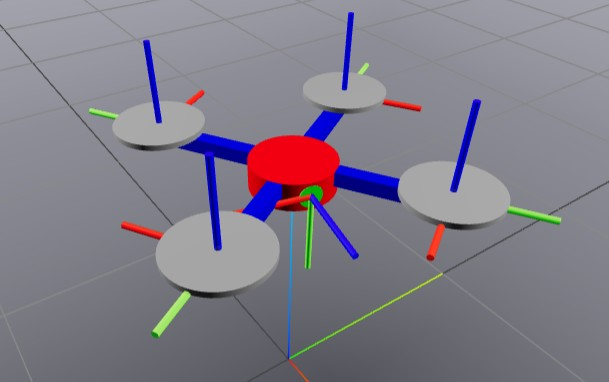
\includegraphics[height=1.5in]{Figures/drone_model.jpg}
        \captionsetup{justification=centering}
        \caption{Implemented quadrotor model with respective rotor propeller frames and front-mounted camera frame.}
        % \label{fig:}
    \end{subfigure}\hfill
    \begin{subfigure}[t]{0.35\textwidth}
        \centering
        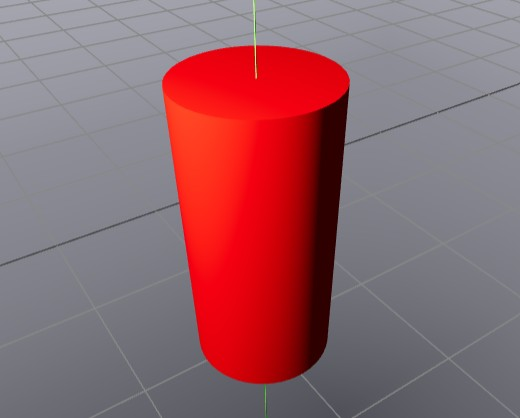
\includegraphics[height=1.5in]{Figures/target_model.jpg}
        \captionsetup{justification=centering}
        \caption{Implemented simple red-cylinder target model.}
        % \label{fig:}
    \end{subfigure}
    \captionsetup{justification=centering}
    \caption{Visualized quadrotor and target model implemented in the Drake simulation.}
    \label{fig:models}
\end{figure}

With the quadrotor and target model loaded into the plant, they, along with the obstacle wall were placed at their initial conditions 
\begin{align*}
    \mathbf x_W^Q(0)&=(-2, -4, 0.5)^T\ m & \psi(0)&=\frac\pi 2\ rad & \mathbf x^T(0)&=(0.5, 5.5, 0.5,1)^T\ m\,,
\end{align*}
as seen in Figure \ref{fig:world_traj}, with all other non-specified initial conditions taken as 0. This image \textit{also} shows a sketch of the planned trajectory of the target during the simulation (from $x_T(0)$ to $(15,-2,0.5)\ m$), in which it will move to the opposite side of the wall as the drone, forcing the drone to continue its tracking even after the target is occluded by the obstacle.

\begin{figure}[htb]
    \centering
    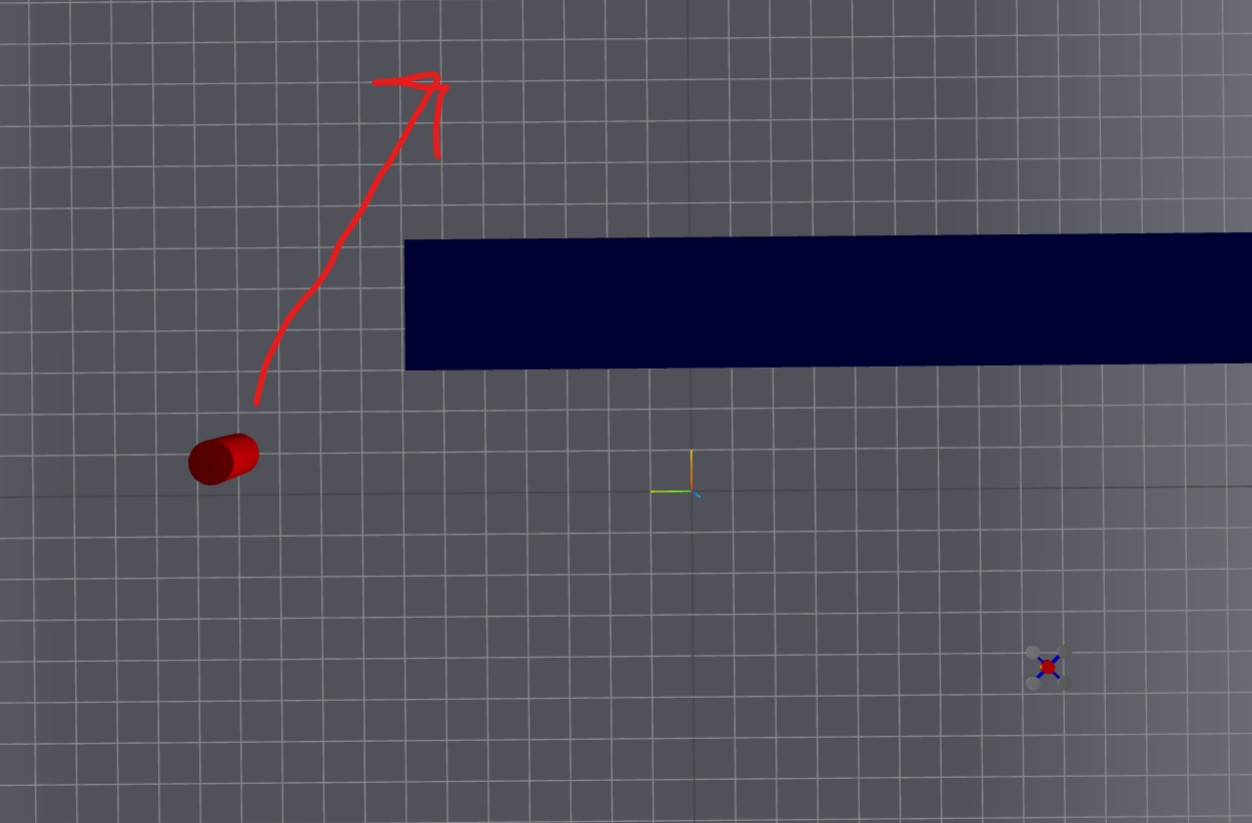
\includegraphics[width=0.5\textwidth]{Figures/world_traj.jpg}
    \captionsetup{justification=centering}
    \caption{Initial Drake simulation configuration of quadrotor, target, and obstacle, as well as a sketch of the planned target trajectory behind the wall.}
    \label{fig:world_traj}
\end{figure}

With the models implemented, the quadrotor RGBD-camera was added into the simulation located at the camera reference frame in Figure \ref{fig:models}, thus providing $T_Q^C$ (\ref{eqn:TQC}). The camera properties implemented were:
\begin{align}\label{eqn:params}
    a&=640\ \text{px} & b&=480\ \text{px} & f_x=f_y&=450\ \text{px} & \text{fps}&=15\ Hz\nonumber\\
    u_0&=a/2\ \text{px} & v_0&=b/2\ \text{px} & z_{min}&=0.1\ m & z_{max}&=20\ m\,,
\end{align}
where $z_{min}$ and $z_{max}$ give the minimum and maximum distance-sensing limits of the RGBD-camera. With these values in (\ref{eqn:params}), $K$ from (\ref{eqn:pT}) and the bounding regions in (\ref{eqn:observe}) are known. 

The TV-LQR controller was then also added to the Drake system, linking the evaluated camera outputs to the quadrotor thrust commands. For the final controller form in (\ref{eqn:fin_control}), cost matrices $Q(k)$ and $R(k)$ were chosen as
\begin{align*}
    Q(k)&=\text{diag}\begin{pmatrix}
        1 & 1 & 100 & 20 & 20 & 20 & 100 & 100 & 100 & 200 & 200 & 200
    \end{pmatrix}\\
    R(k)&=\text{diag}\begin{pmatrix}
        1 & 1 & 1 & 1 
    \end{pmatrix}\,,
\end{align*}
where ``diag$(\cdot)$'' is the diagonalization operator that turns a vector into a diagonal matrix. These costs were chosen to penalize high quadrotor velocities, which can cause ``jerky'' motions and cause the target to fall out of view of the quadrotor. The desired reference offset values for quadrotor tracking were
\begin{align*}
    \delta_x(k)&=-2\ m & \delta_y(k)&=2\ m & \delta_z(k)&=0\ m\,.
\end{align*}

\subsection{DRAKE SIMULATION EVALUATION}
With the Drake system completed, it was simulated from $t\in[0,10]\ s$, with simulation data ($\mathbf x_W^Q,\mathbf x_T,\mathbf v_T,\mathbf x_T^e,\mathbf v_T^e,(x_Q^r,y_Q^r,z_Q^r),(u,v),(u^e,v^e)$) captured at every frame of the quadrotor's camera, such that $\Delta t=1/\text{fps}=1/15\ s$. Additionally, each frame of the RGBD-camera was exported and compiled into a video with specific overlays added on top. Notably, the true target pixel positions $(u,v)$ in the camera image plane, the estimated target pixel positions $(u^e,v^e)$ in the camera image plane, and the calculated bounding box from (\ref{eqn:boundingbox}) were added to each frame for visual clarity (shown in Figure \ref{fig:sample_frames}). These results were then logged upon the simulation's completion for analysis and observation.

\section{RESULTS}\label{sec:results}
Figure \ref{fig:target_pixels} shows the plot of $(u,v)$ and $(u^e,v^e)$ versus time. As seen, with the bounding box object detection approach explored in Section \ref{sec:theory}, the quadrotor was able to accurately estimate the target's pixel coordinates through bounding box construction. The target was occluded by the wall from $t\sim[3,4]\ s$, and even after that occlusion, the drone was still able to regain the target in its sensor FOV and continue tracking it throughout the target's trajectory. The brief ``dip'' at the beginning is caused by the target not yet being found on the initial frame, which caused the quadrotor to begin moving towards the initially defined reference position (the world origin) rather than the target, causing it to tilt down and move until the target was registered in frame.

\begin{figure}[htb]
    \centering
    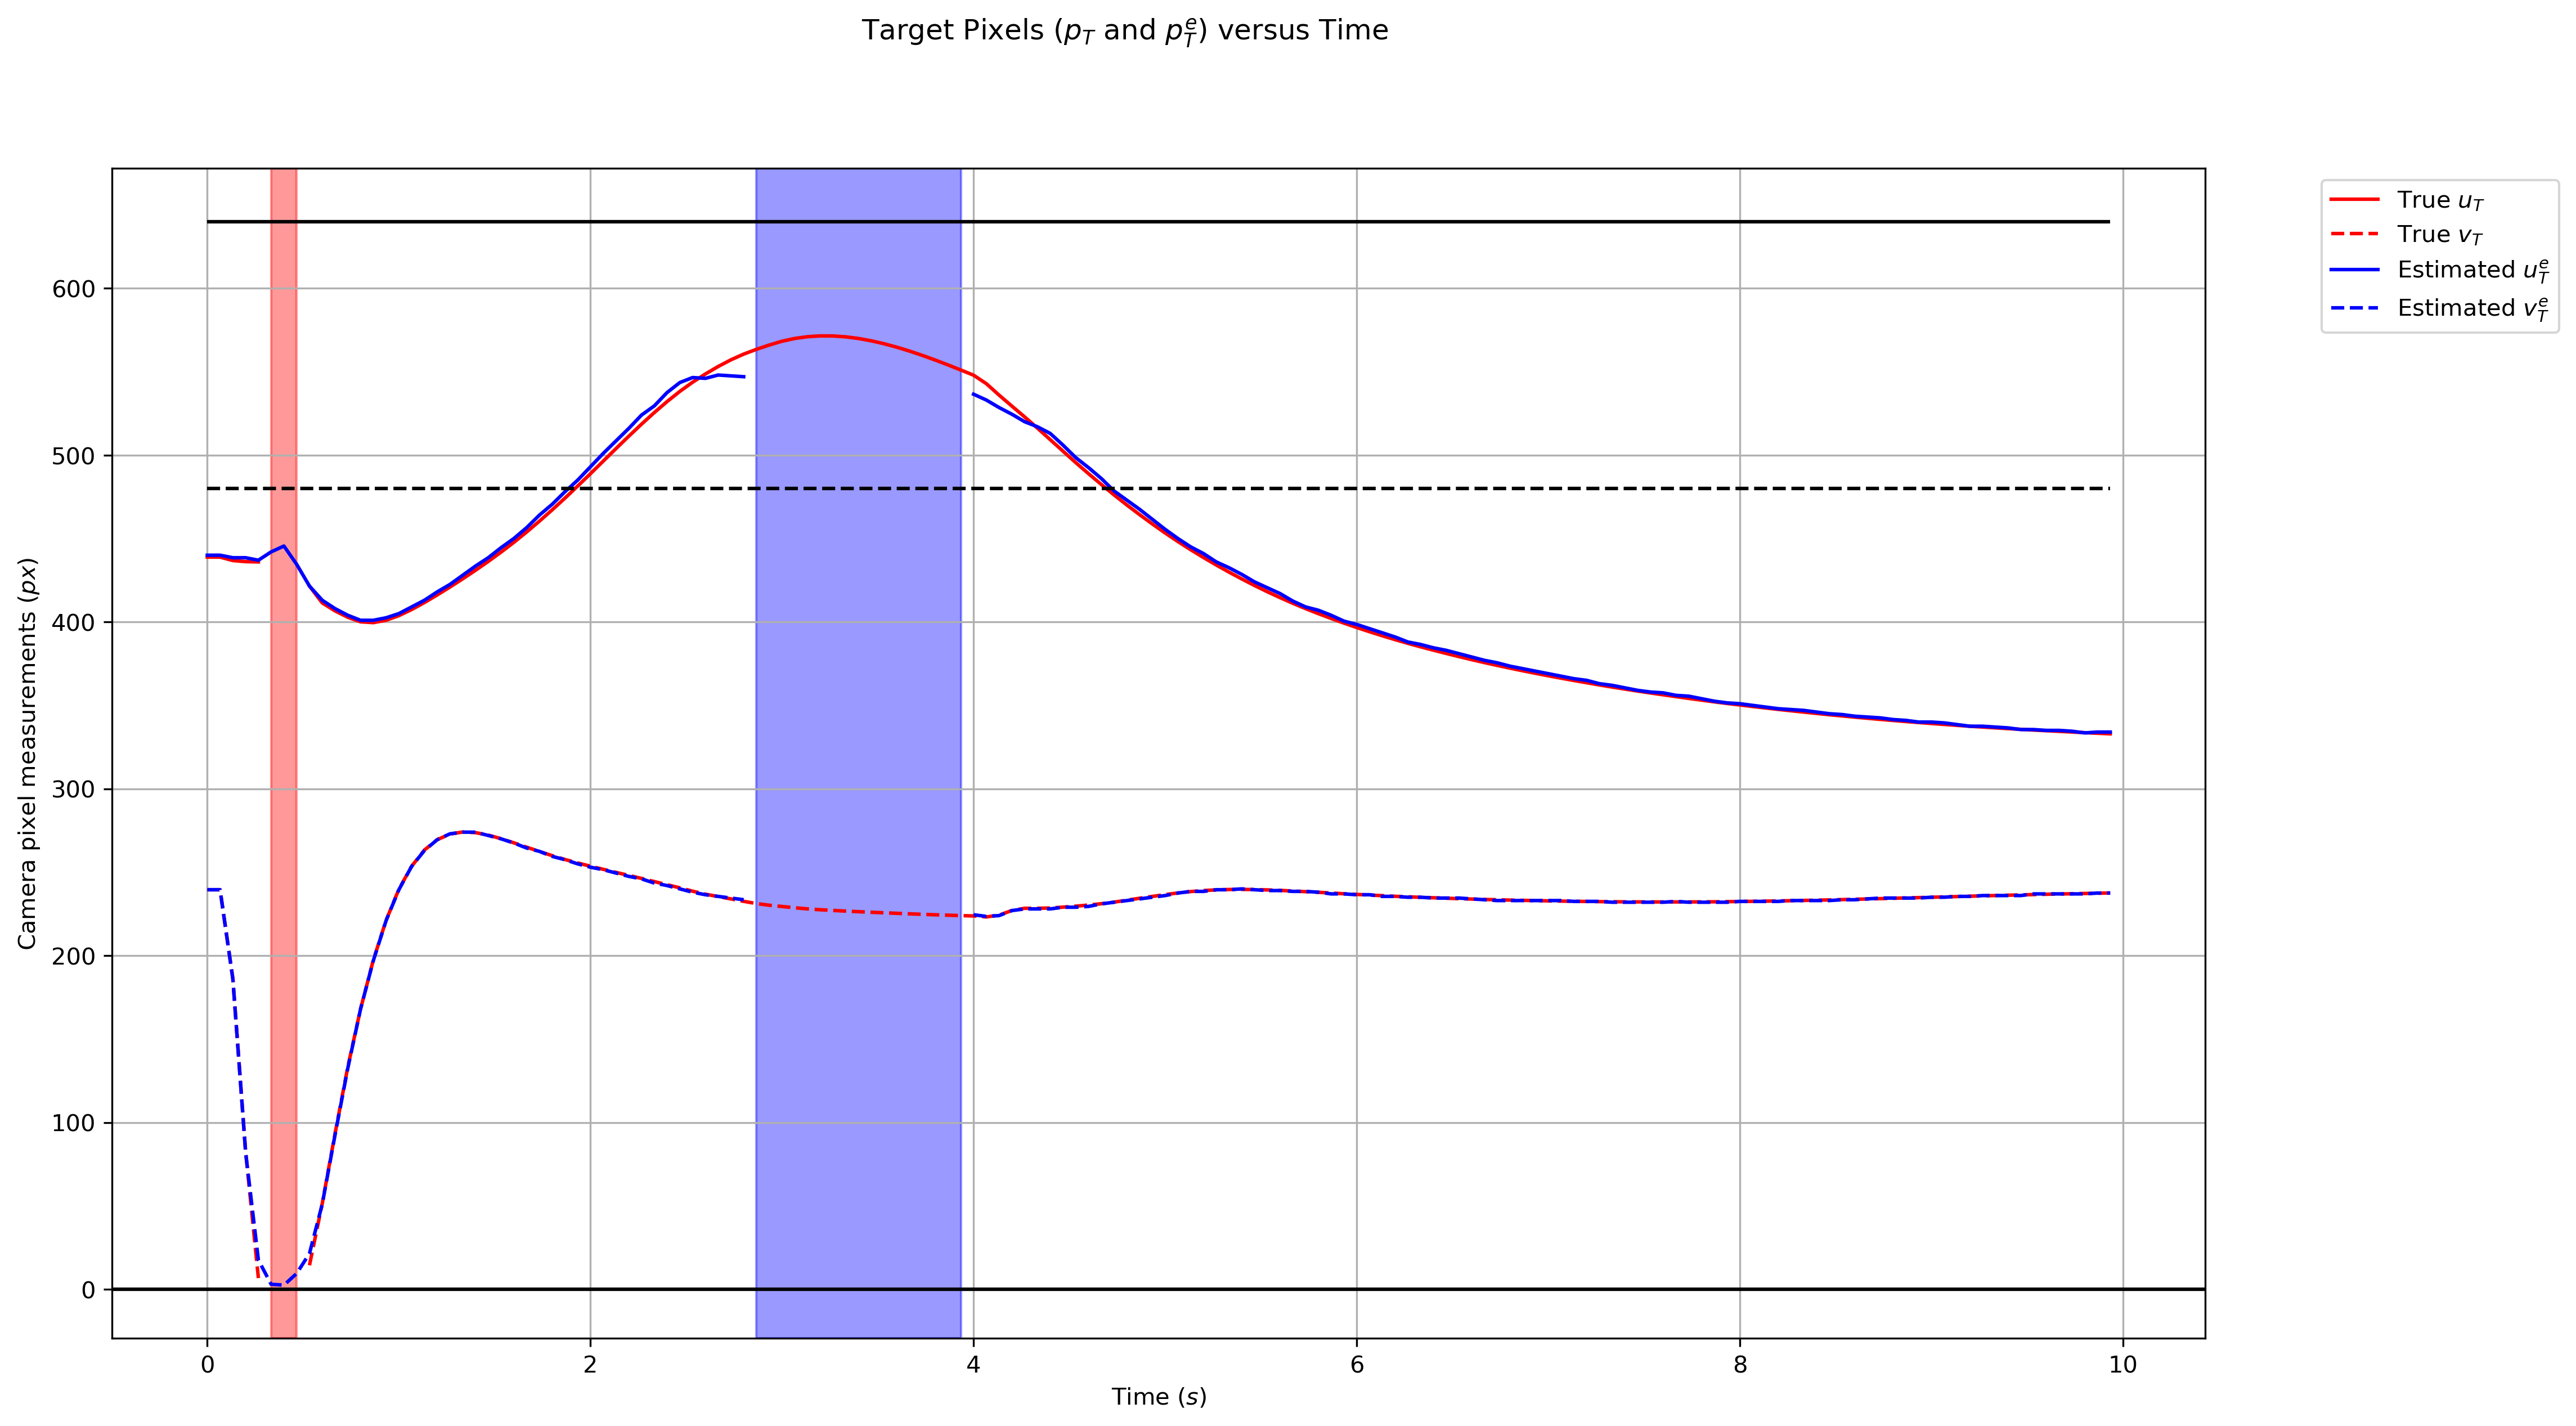
\includegraphics[width=0.6\textwidth]{Figures/target_pixels.png}
    \captionsetup{justification=centering}
    \caption{Plot of $(u,v)$ from (\ref{eqn:pixels}) and $(u^e,v^e)$ from (\ref{eqn:uve}) versus time, with black lines denoting camera bounding limits, red regions denoting times when the target's COM was \textit{theoretically} out of frame and blue regions denoting when no target estimated pixels were found due to environmental occlusions.}
    \label{fig:target_pixels}
\end{figure}

To demonstrate when the target was able to be realized withing the RGBD-sensor versus when it was occluded, Figure \ref{fig:sample_frames} displays two frames taken from the augmented video of the camera feed. As seen, when the target is within the frame, the estimated $(u^e,v^e$) position aligns visibly well with the true $(u,v)$ results, skewed by the imperfect target bounding box/masking, which is affected by the ambient lighting and shadows, as well as the current orientation of the quadrotor (a tilted quadrotor will cause the bounding box region to not perfectly encompass the target).

\begin{figure}[htb]
    \centering
    \begin{subfigure}[t]{0.5\textwidth}
        \centering
        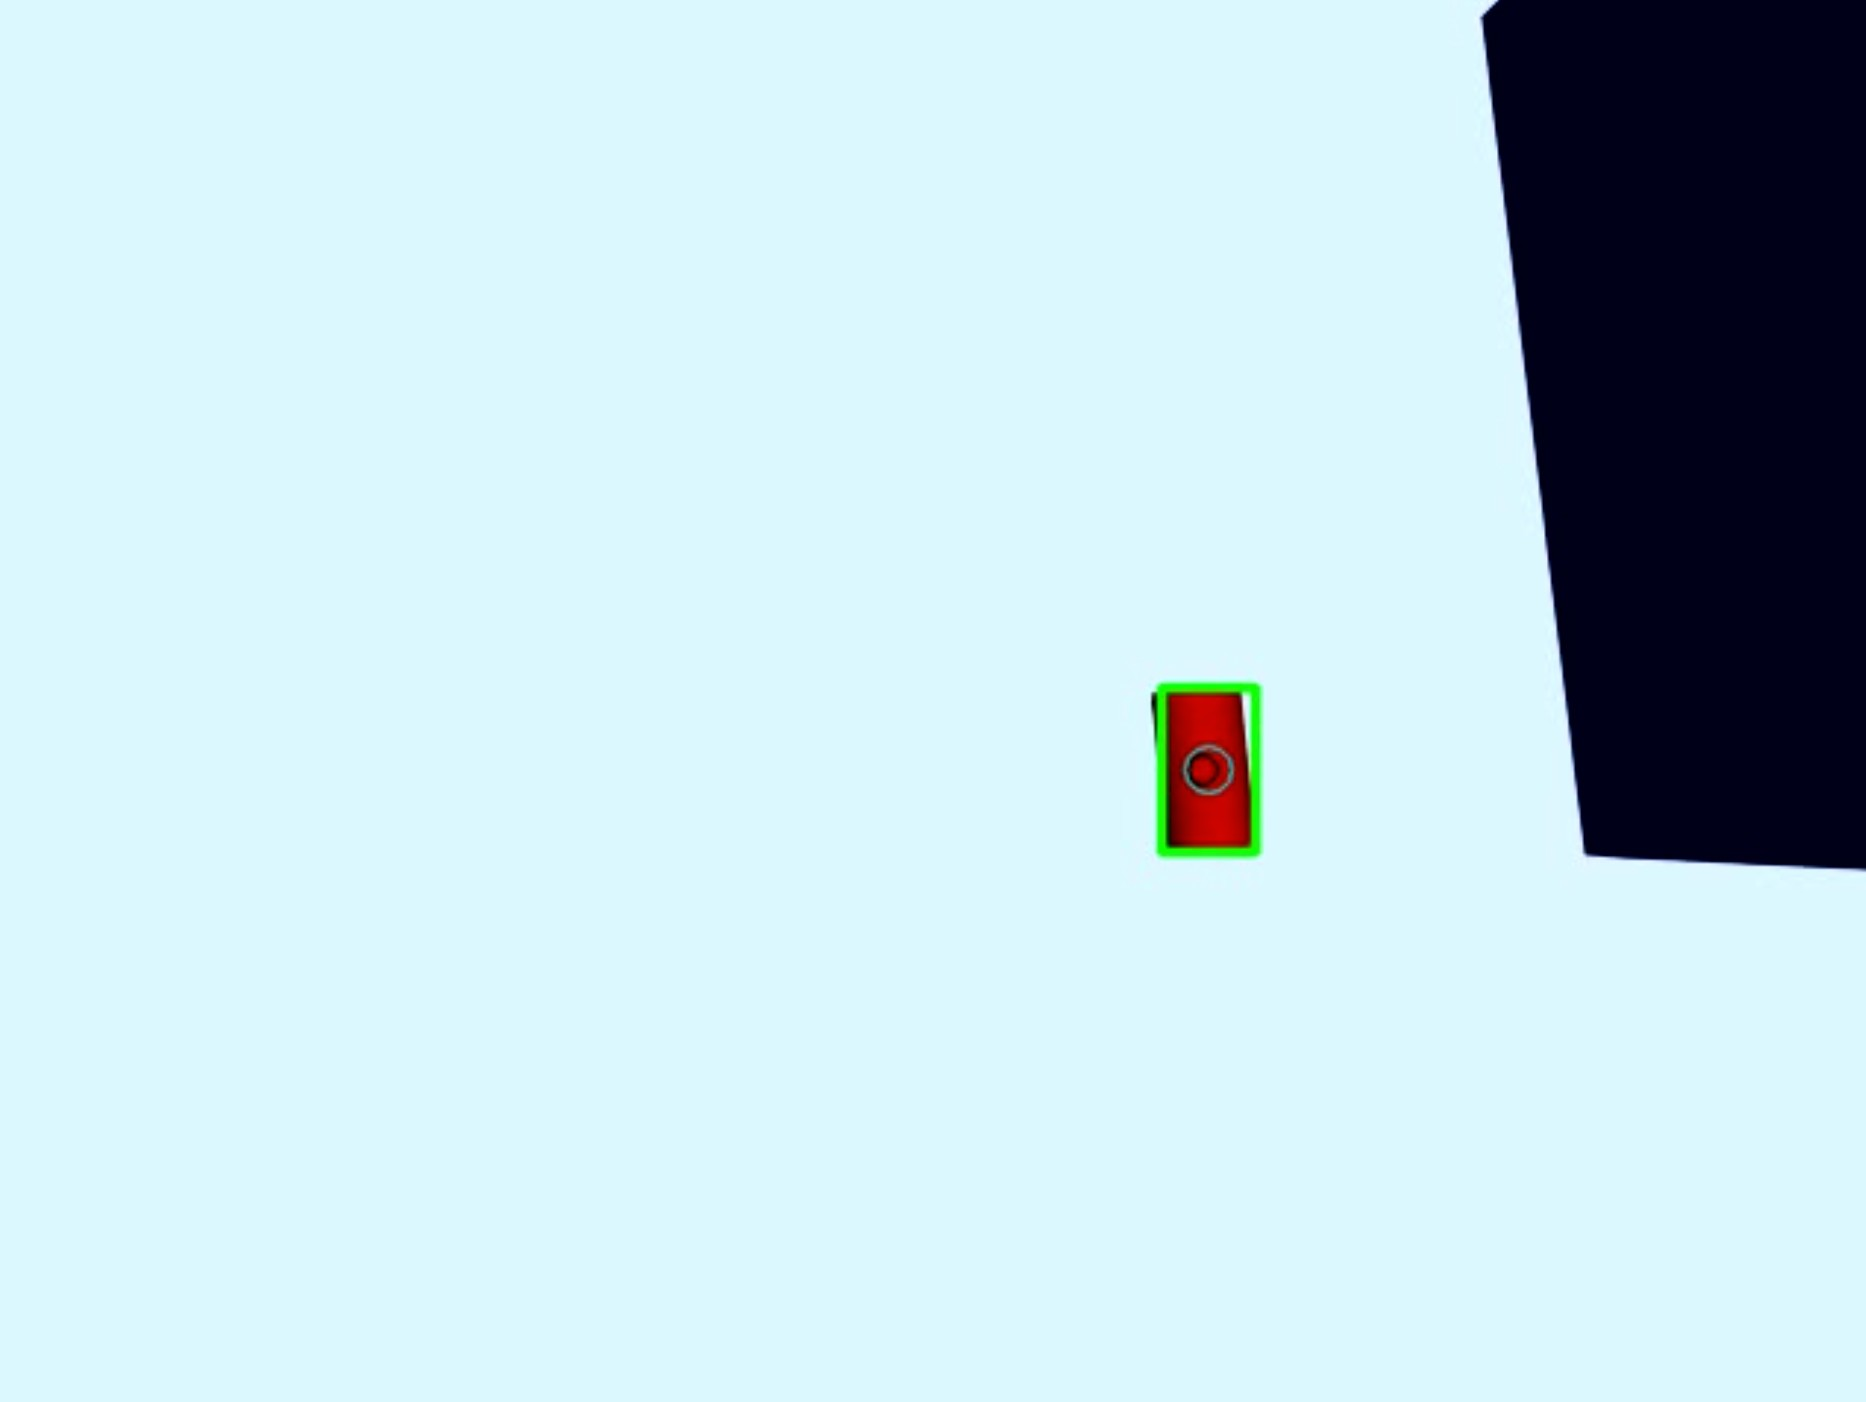
\includegraphics[width=0.8\textwidth]{Figures/sample_frame.jpg}
        \captionsetup{justification=centering}
        \caption{Target found within sensor region ($t\approx 1\ s$).}
        % \label{fig:}
    \end{subfigure}\hfill
    \begin{subfigure}[t]{0.5\textwidth}
        \centering
        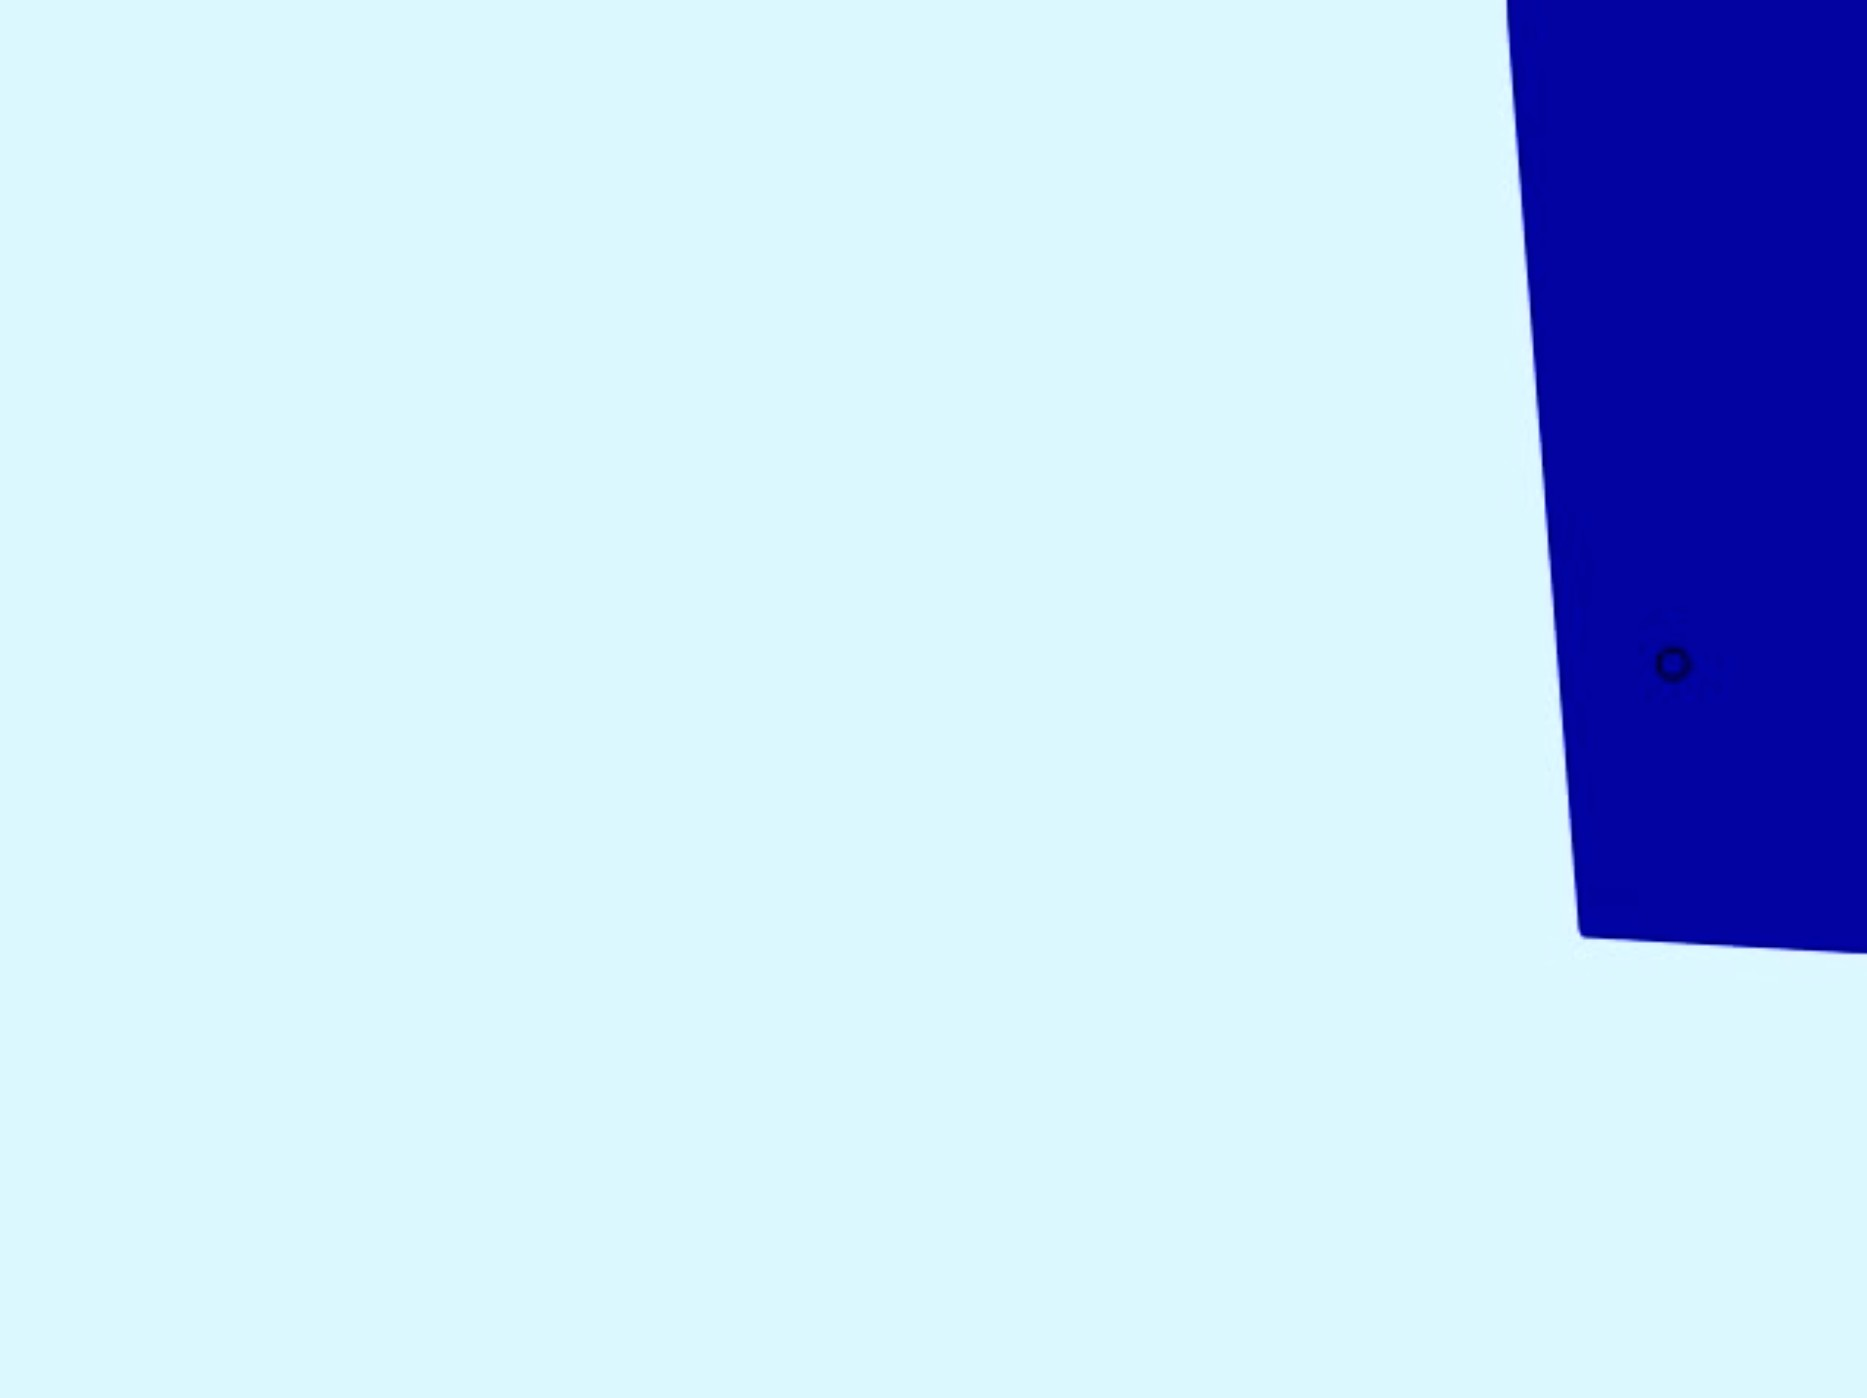
\includegraphics[width=0.8\textwidth]{Figures/sample_frame_blocked.jpg}
        \captionsetup{justification=centering}
        \caption{Target occluded from sensor by the environmental obstacle ($t\approx 3\ s$).}
        % \label{fig:}
    \end{subfigure}
    \captionsetup{justification=centering}
    \caption{Augmented frames from the quadrotor's RGBD-sensor showing the true target COM $(u,v)$ (black circle), the estimated target COM $(u^e,v^e)$ (cyan circle), and determined bounding box of the target through the sensor measurement and estimation models.}
    \label{fig:sample_frames}
\end{figure}

Figure \ref{fig:target_state} shows a plot of the estimated target \textit{position} $\mathbf x_T^e$ from (\ref{eqn:uve}), (\ref{eqn:we}), and (\ref{eqn:inverse}), and estimated target \textit{velocity} $\mathbf v_T^e$ from (\ref{eqn:vTe}) along with the tre values, respectively. As seen, outside of the occluded regions and the initial ``dip'' at the beginning (explained earlier), both the target \textit{positions} were able to be estimated accurately, with more noise present in the estimated target velocities. As seen, in the occluded regions, while $\mathbf x_T^e$ vanishes, $\mathbf v_T^e$ persists, as it is stored to estimate the dynamics of the target in (\ref{eqn:update_dyn}) to the last measured value. Of the estimates, those corresponding to the global $y$-axis are the least accurate. The reason for this is due to the bounding box object detection approach. When the target is \textit{partially} occluded by the obstacle, the bounding box becomes thin, and the estimated $(u^e,v^e)$ shifts away from the target's true COM towards the side that is still visible. This causes the respective direction $(y)$ to drift away from the true and imposes an artificial ``velocity'' as the estimated COM ``moves'' in the camera frame, even if no such movement actually occurs. That is why the estimated $y$ velocity of the target increases directly before the target is fully occluded.  

\begin{figure}[htb]
    \centering
    \begin{subfigure}[t]{0.5\textwidth}
        \centering
        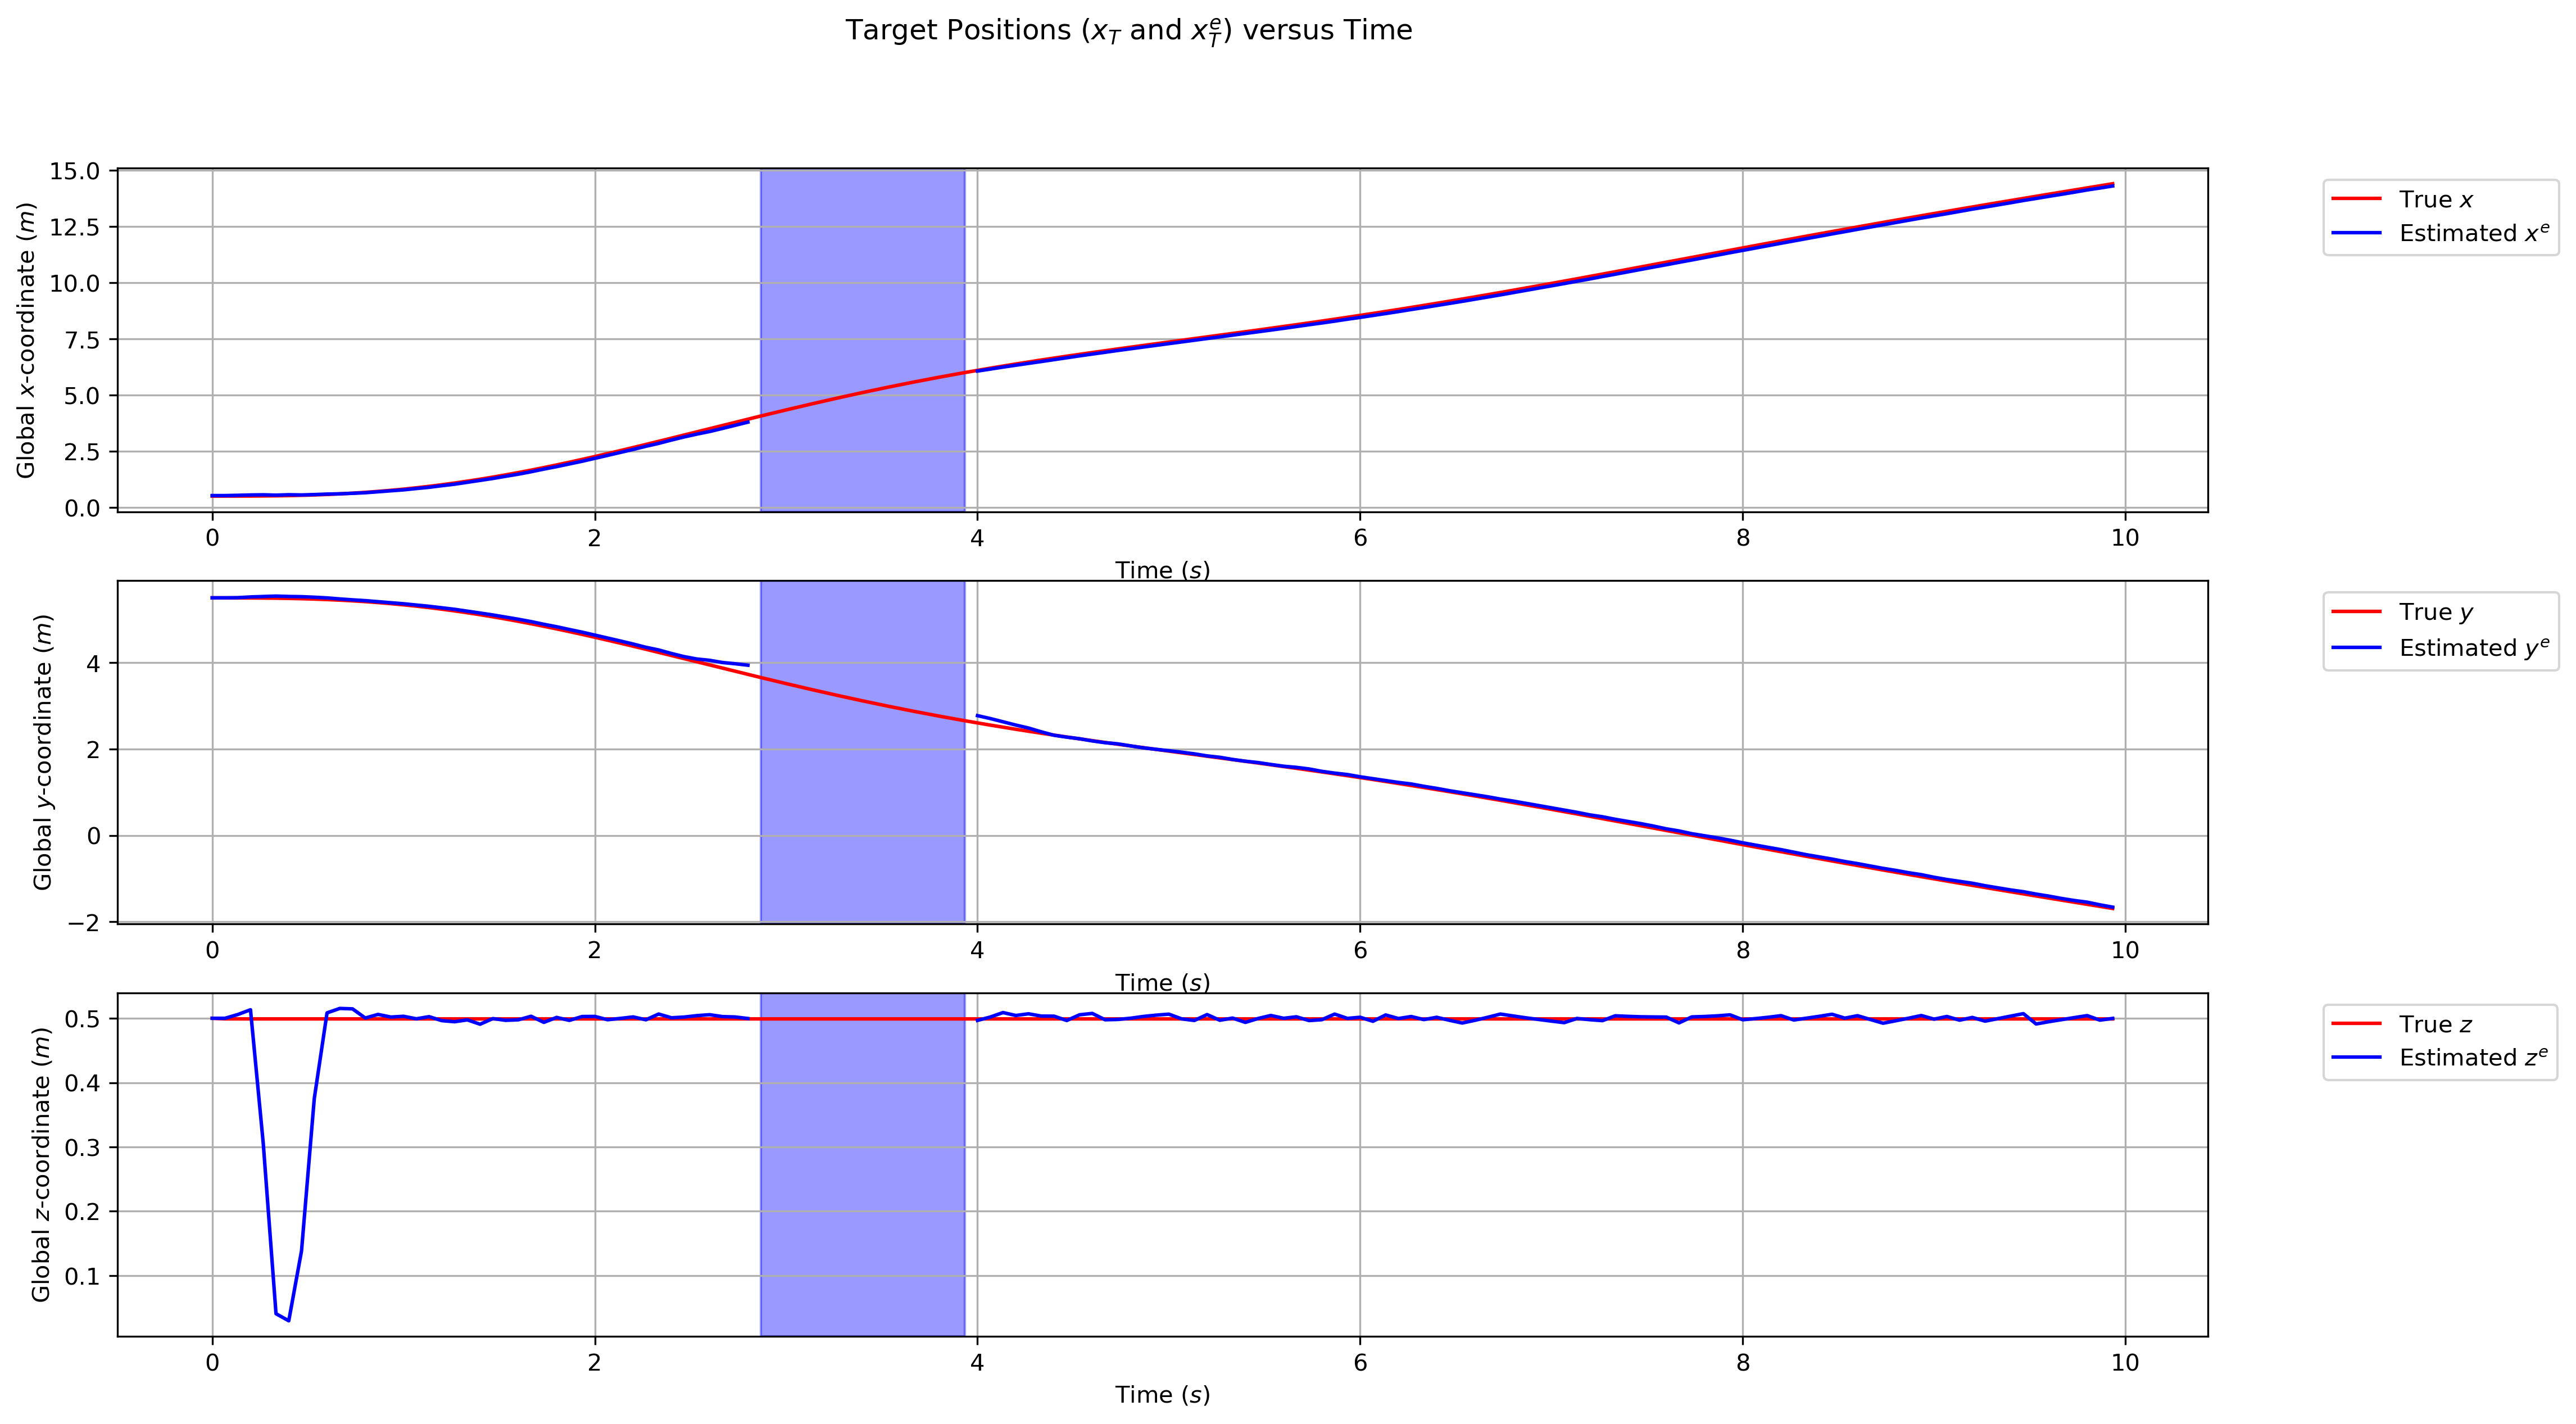
\includegraphics[width=0.9\textwidth]{Figures/target_positions.png}
        \captionsetup{justification=centering}
        \caption{True target position $\mathbf x_T$ overlayed with estimated target position $\mathbf x_T^e$ in the global $x$, $y$, and $z$ coordinates.}
        % \label{fig:}
    \end{subfigure}\hfill
    \begin{subfigure}[t]{0.5\textwidth}
        \centering
        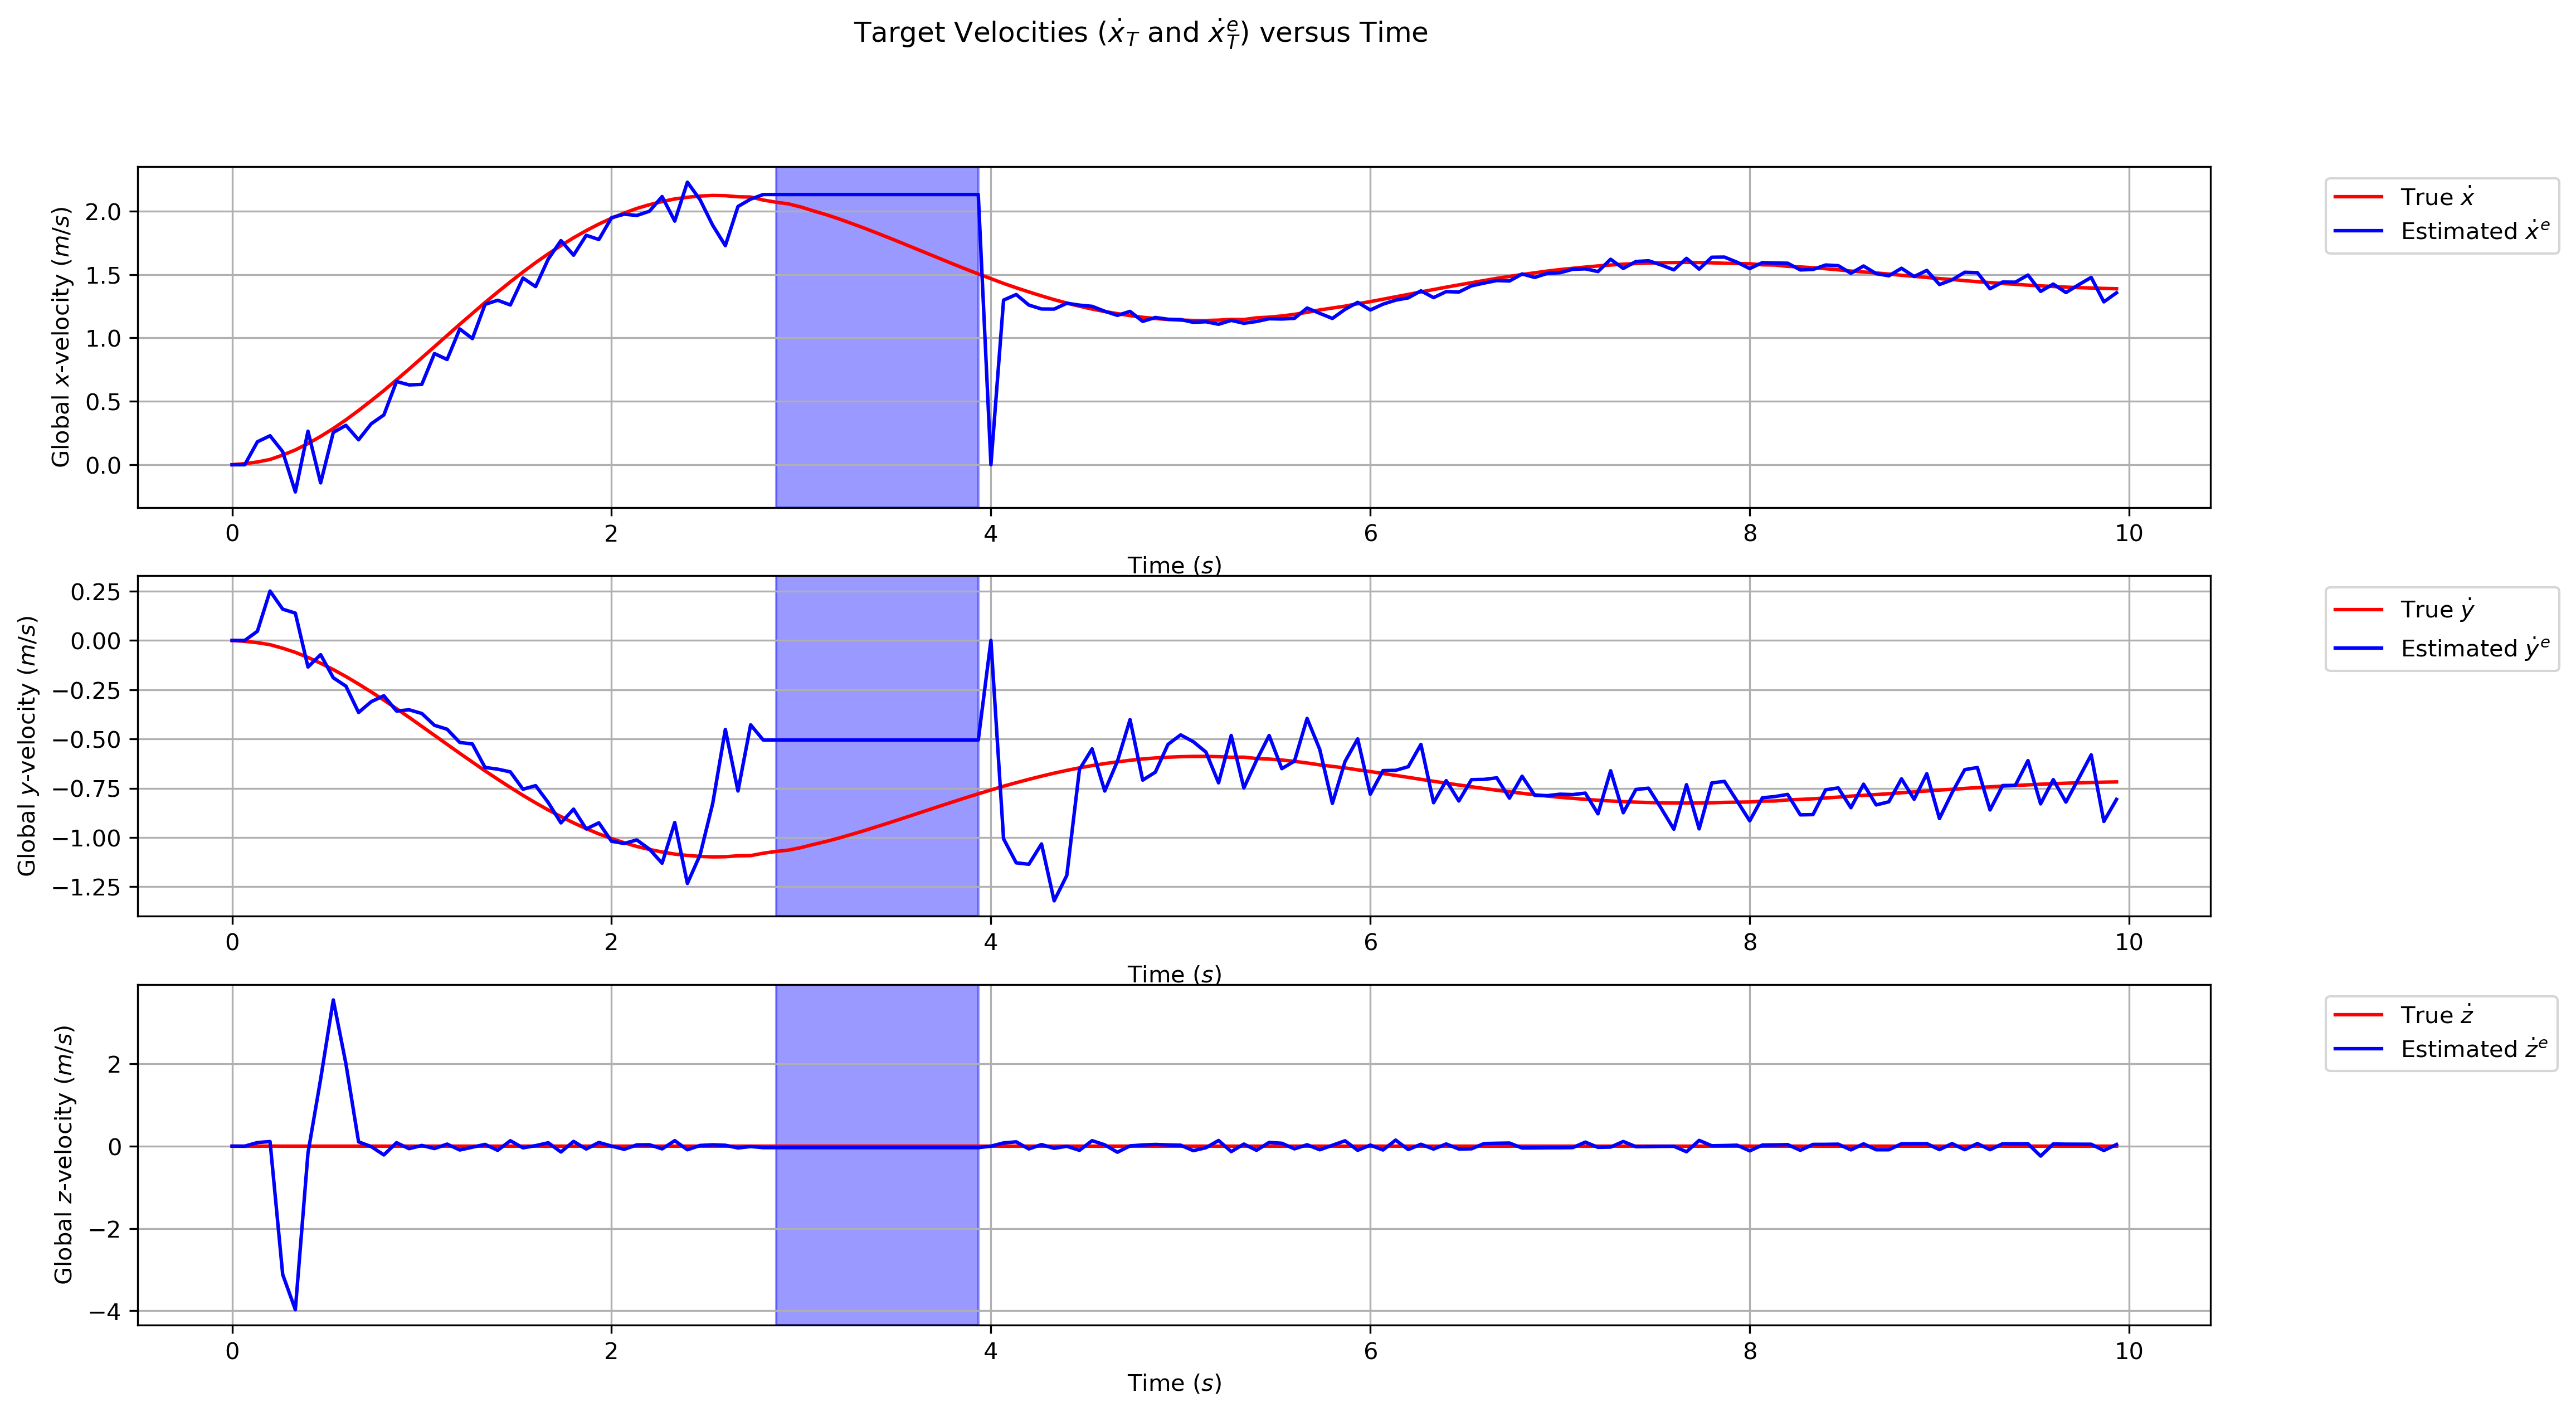
\includegraphics[width=0.9\textwidth]{Figures/target_velocities.png}
        \captionsetup{justification=centering}
        \caption{True target velocity $\mathbf v_T$ overlayed with estimated target velocity $\mathbf v_T^e$ in the global $x$, $y$, and $z$ coordinates.}
        % \label{fig:}
    \end{subfigure}
    \captionsetup{justification=centering}
    \caption{Comparison of true target state ($\mathbf x_T,\mathbf v_T$) and estimated target state from quadrotor RGBD-camera measurements ($\mathbf x_T^e,\mathbf v_T^e$), with blue regions showing where the target was occluded by the obstacle.}
    \label{fig:target_state}
\end{figure}

Finally, to illustrate the optimal tracking and dynamical estimation of the target's position, Figure \ref{fig:drone_reference} shows the quadrotor's position $\mathbf x_W^Q$, the estimated target position $\mathbf x_T^e$, and calculated reference position from (\ref{eqn:qr}) and (\ref{eqn:update_dyn}) for the TV-LQR controller input (\ref{eqn:fin_control}). As seen, even when the target's estimated position is missing due to occlusions, the quadrotor's tracking reference was continually updated through the estimated target dynamical model, thus allowing it to continue tracking the target even through the occlusion. Then, after the target was regained within the sensor's FOV, the reference updated to the new estimated target position for the controller. While it may appear that the drone is tracking ``poorly'' due to the offset between the desired reference position and the actual position, this is simply a matter of tuning the controller gains $Q(k)$ and $R(k)$. As previously mentioned, the gains were chosen to minimize quadrotor velocities so that it can maintain the target in view and minimize sudden movements. If these velocities were punish less with respect to the positional gains, then the quadrotor position would converge to the reference position more rapidly, at the cost of more potential ``dips'' as seen at the beginning of the $z$-coordinate plot from the tilting motion of the quadrotor.

\begin{figure}[htb]
    \centering
    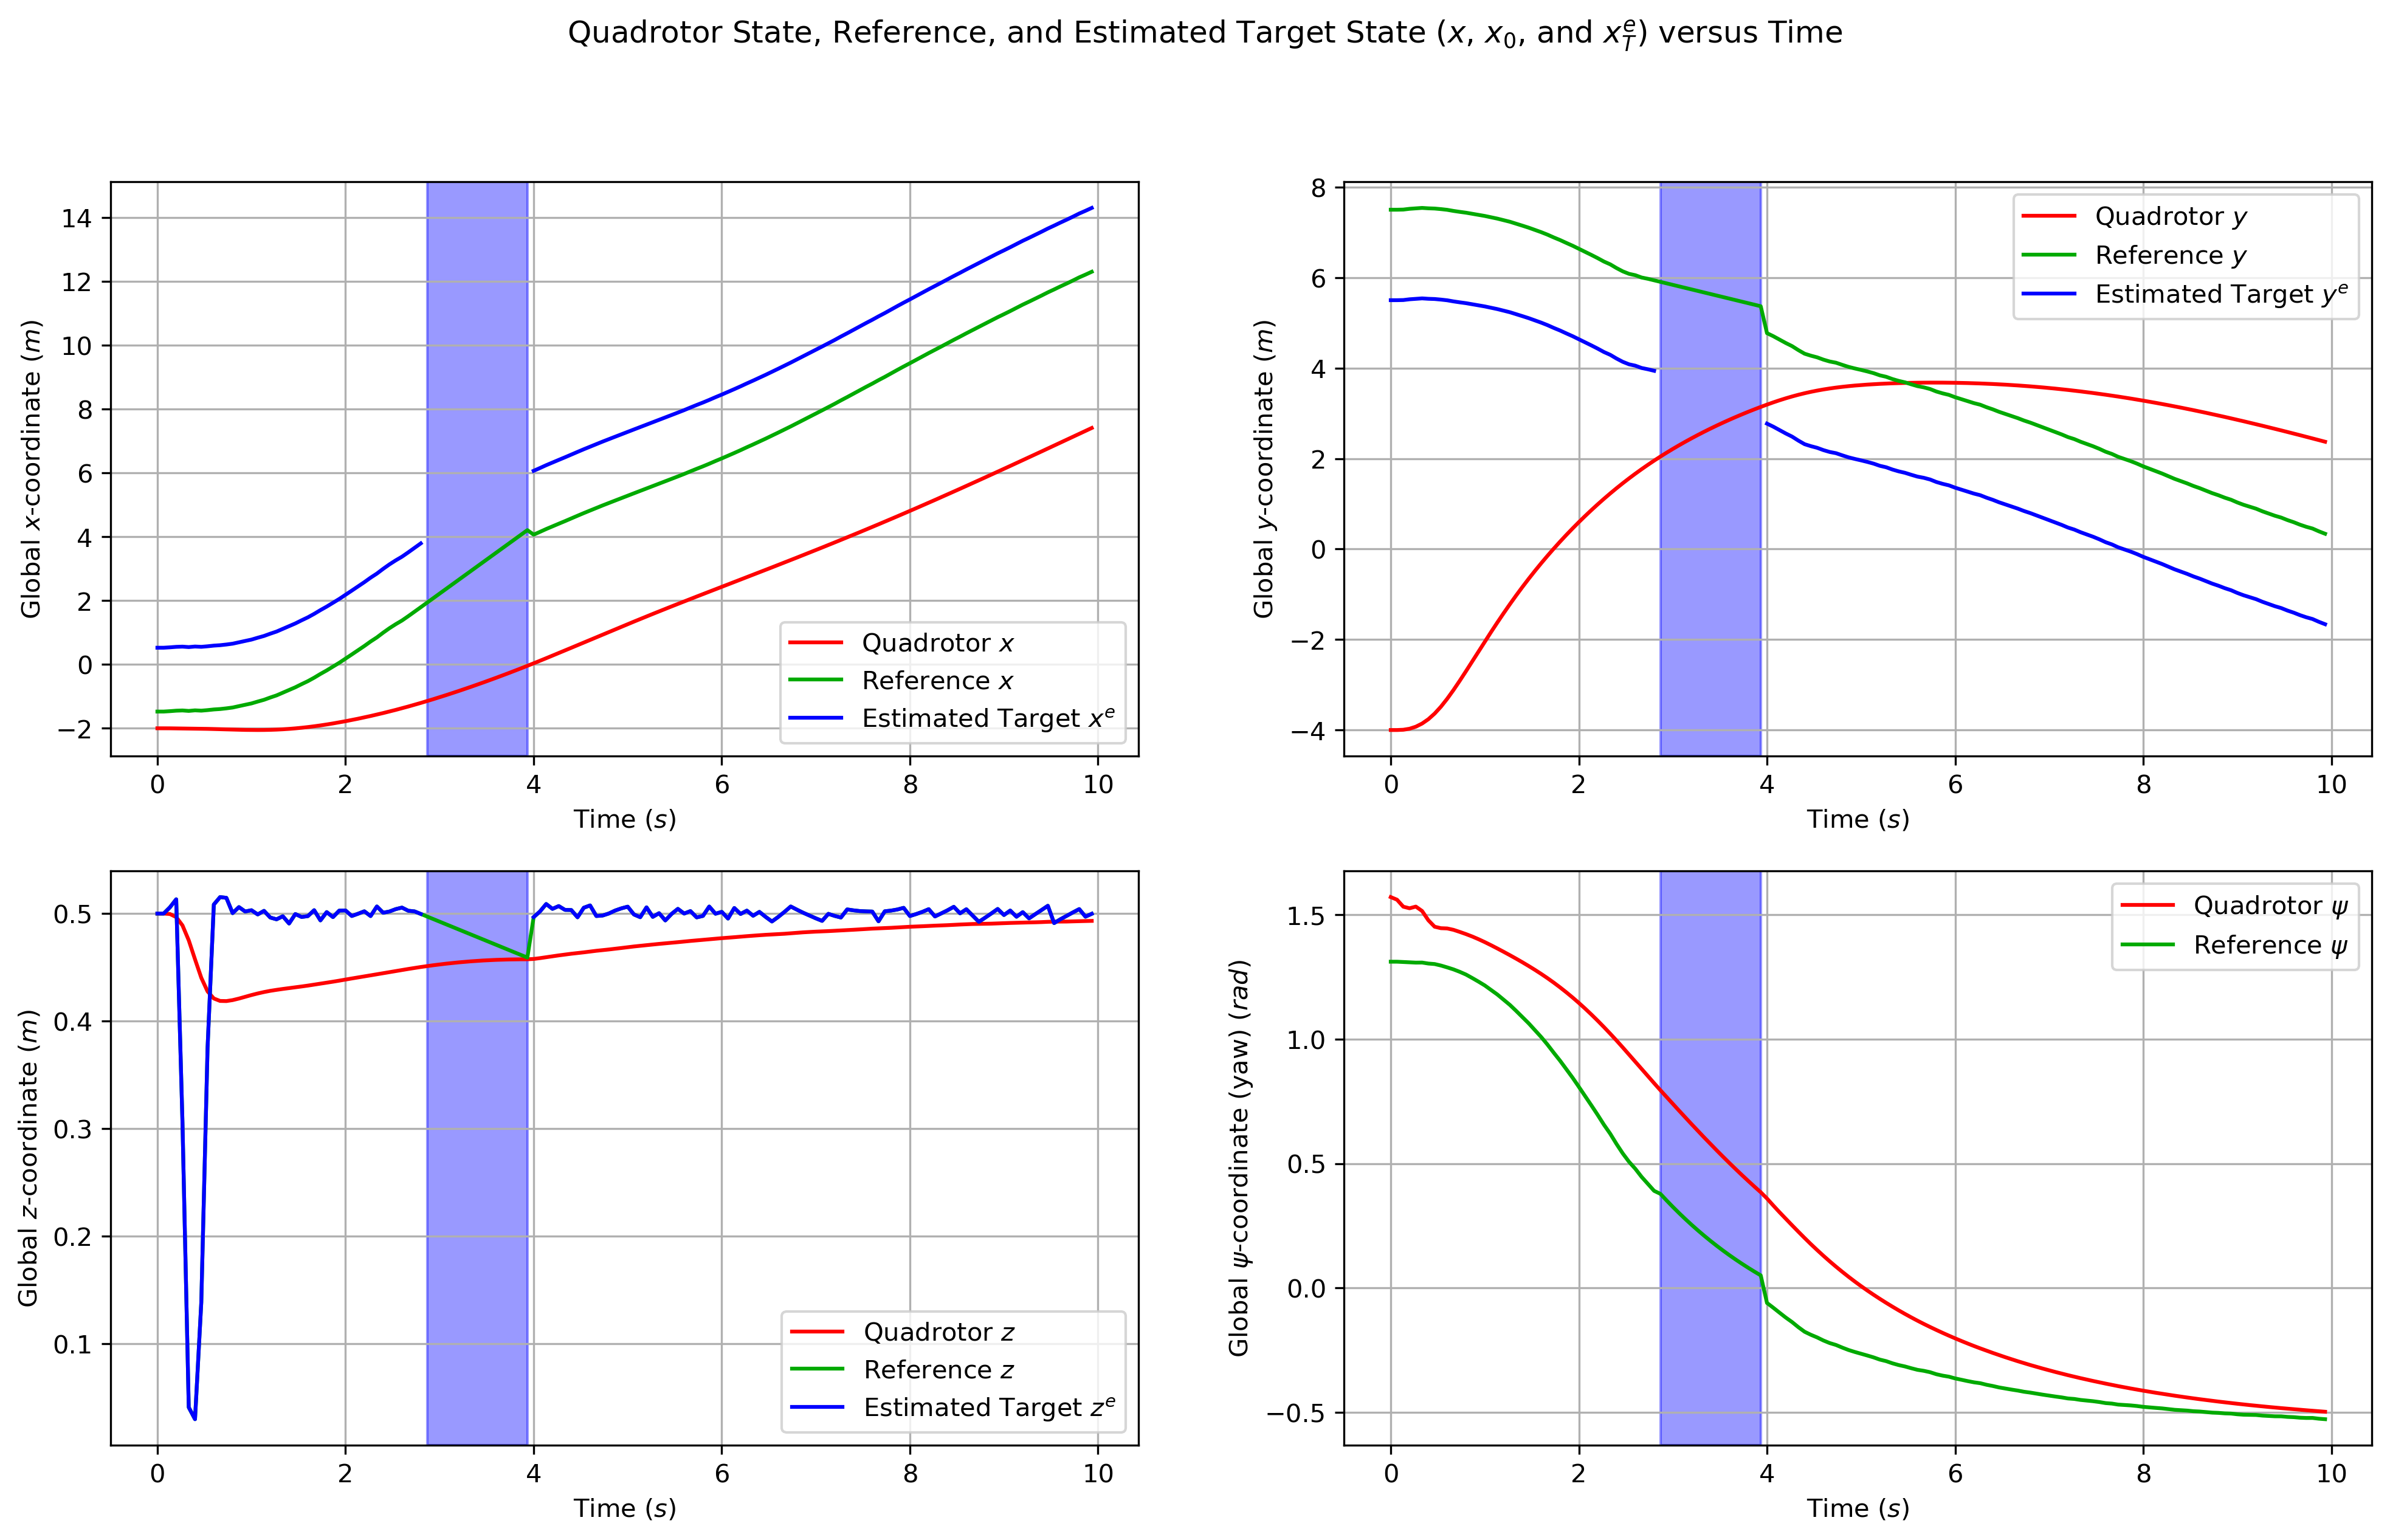
\includegraphics[width=0.7\textwidth]{Figures/drone_reference.png}
    \captionsetup{justification=centering}
    \caption{Plot of quadrotor $\mathbf x_W^Q$, $\mathbf x_T^e$, and $(x_Q^r,y_Q^r,z_Q^r,\psi^r)$ showcasing the dynamical estimation of the target through the updating reference, as well as the optimal tracking control performance.}
    \label{fig:drone_reference}
\end{figure}

The source link to the complete simulation code can be found in Appendix \ref{app:code}, which also contains the complete augmented video file of the quadrotor's RGBD-camera frames, as well as an overhead video of the simulated drone/target/obstacle system. While the demonstrated results utilizing the mathematical models in Section \ref{sec:theory} showcase that the quadrotor was able to perform active perception tracking for a target using object detection and estimation mechanisms, the results are still not perfect. The biggest source of noise is in the target state estimation method, which uses a bounding box algorithm for the position and first-order discretization for the velocity. While optical flow was disregarded for velocity estimation, it can be \textit{combined} with the discretized estimation to reduce the uncertainty in the results. Additionally, when generating the bounding boxes, the actual rotation of the quadrotor can be accounted for, thus ``rotating'' the target to align with the camera's reference frame so that the bounding box always aligns vertically with the target, reducing this source of ``jitter'' error. Another source of error is in the actual tracking itself. As mentioned, the gains were chosen to minimize velocity, but for a more aggressive quadrotor or tracking mission, it may need to maintain its reference state much more closely. For this, while the gains can be tuned differently, another approach is for the velocity coordinates of $\mathbf q_Q^r$ to be set as the estimated target velocities, although this would require more sophisticated trajectory reference generation, as $\mathbf u_Q^r$ would then need to be calculated based on the desired velocities.

\section{CONCLUSIONS}\label{sec:conclusion}
This project sought to mathematically model a quadrotor-RGBD-camera system and use it to perform active perception by optimally tracking and following a desired target with a discrete TV-LQR controller, maintaining an estimated dynamic model of the target to update its reference trajectory even through environmental occlusions. While the current model is functional as is, there is, of course, still much room for future improvement. First, the quadrotor can only track a single target. As soon as there are multiple targets and bounding boxes, it may not stay ``connected'' to the desired target as it relies solely on the maximum ``contourArea'' of the found bounding boxes to discriminate. If, for example, another target grows ``larger'' than the desired target (by moving near the quadrotor), then the system will switch to tracking the undesired target. More sophisticated target/object detection schemes can solve this, as well as the implementation of optical flow to ensure that the bounding box stays within a certain threshold of the desired target's optical flow region. Second, the target in this simulation was a simple red cylinder, which, for proof of concept, made for simple object detection in a plain environment, but for a more complex sensor measurement image, more sophisticated object detection algorithms should be implemented (with CNNs, perhaps). Thirdly, while the obstacle occlusion \textit{does} affect the quadrotor's sensor measurements and estimations of the targets, the quadrotor is not currently detecting the target and storing related information about it. Therefore, there is a chance, based on how the target moves, that the quadrotor simply collides with the obstacle in its trajectory towards the target, which is not ideal. To remedy this, the quadrotor can also perform object detection on obstacles and implement their estimated positions into its optimal control law to avoid collisions while still maintaining tracking. 

%%%%% REFERENCES
\clearpage
\printbibliography[title={\textbf{REFERENCES}}]

%%%% APPENDIX
\appendix\appendixpagenumbering
\section{SIMULATION CODE}\label{app:code}
For the complete simulation code and results (including the complete video output), refer to the following GitHub repository:

\href{https://github.com/dan-whitman/Courses/tree/main/MAE%205810/Mid-Final%20Project}{https://github.com/dan-whitman/Courses/tree/main/MAE 5810/Mid-Final Project}

\end{document}
